\documentclass[a4paper,11pt]{article}
\usepackage[english]{babel}
\usepackage[utf8]{inputenc}
\usepackage[T1]{fontenc}
\usepackage{graphicx}
\usepackage{amsmath}
\usepackage{tikz}
\usepackage{amsthm}
\usepackage{amssymb}
\usepackage{nicefrac}
\usepackage{tabularx}
\usepackage{cprotect}
\usepackage{wrapfig}
\usepackage{framed}
\usepackage{fancyvrb}
\usepackage{bm}
\usepackage{listings}
\usepackage{longtable}
\usepackage[left=25mm,right=25mm,bottom=25mm,top=25mm]{geometry} %left, right, bottom ,top, includeheadfoot
\usepackage{caption}
\usepackage{multicol}
\usepackage{subcaption}
\usepackage{nameref}
\usepackage{placeins} %Put command \floatbarrier in front of textpassage or other items, in front of which the desired content (i.e. images) shall be placed.
\usepackage[inline]{enumitem}
% \usepackage[parfill]{parskip}
%\usepackage{fancyhdr}
\usepackage{enumitem}
\usepackage{siunitx}
\newcounter{question}
\setcounter{question}{0}
\usepackage{blindtext}
\usepackage{hyperref} %To make document linked within.
\usepackage{cleveref}
\numberwithin{equation}{section}
\captionsetup{font=footnotesize,labelfont=bf}

\lstset{
	language=Python,
	backgroundcolor=\color{white},   % background color
	basicstyle=\ttfamily\small,      % basic font style
	breaklines=true,                 % automatic line breaking
	basicstyle=\ttfamily\tiny,      % smaller font size (footnotesize)
	postbreak=\mbox{\textcolor{red}{$\hookrightarrow$}\space},  % symbol for line break
	frame=single,                    % frame around the code
	keywordstyle=\color{blue},        % keywords in blue
	commentstyle=\color{green},      % comments in green
	stringstyle=\color{red},         % strings in red
	showstringspaces=false,          % don't show space symbol
	numbers=left,                    % line numbers on the left
	stepnumber=1,                    % step for line numbers
	numberstyle=\tiny\color{gray},   % line numbers in gray
	numbersep=5pt                    % distance between line numbers and code
}

\renewcommand{\theenumi}{(\arabic{enumi})}
\renewcommand\labelenumi{\theenumi} % Change enumerate style from 1. to (1) etc.
\renewcommand{\theenumiii}{(\arabic{enumiii})}
\renewcommand\labelenumiii{\theenumiii} % Change enumerate style from 1. to (1) etc.
\setlist{itemsep = 0.2pt}


\newcommand\matr[1]{\ensuremath{\boldsymbol{\mathbf{#1}}}}
\newcommand\vect[1]{\ensuremath{\bm{#1}}}
\newcommand\dint{\ensuremath{\int\displaylimits}}

%\DeclareSIUnit \parsec {pc}
%\DeclareSIUnit \magnitudes {mag}
\DeclareSIUnit \curie {Ci}

\title{Finite Element Analysis\\ \vspace{0.2cm}\normalsize Questions and Answers}
\author{Daniel Zahnd}
\date{\today}


\newtheorem{ass}{Assertion}

\begin{document}


\newcommand\Que[1]{%
   \leavevmode\par
   \stepcounter{question}
   \noindent
   \thequestion. \textbf{Q} --- #1\par}

\newcommand\Ans[2][]{%
    \leavevmode\par\noindent
   {\leftskip0pt
    \textbf{A} --- \textbf{#1}#2\par}}

\maketitle
%\thispagestyle{empty}
\tableofcontents
%\newpage

\pagenumbering{arabic}
\setcounter{page}{1}

\section{Preliminaries}
\Que{What are the basic requirements of a good finite elements simulation?}
\Ans{
In order to obtain a good finite element model, the geometry of the problem, the involved forces and the material properties need to be known and clear. For example, the geometry of a beam, the applied stress (forces) and the material properties of the beam need  to be known to properly simulate the bending under application of some force.
}

\Que{What is the finite element method?}
\Ans{
The finite element method is a way to numerically solve partial differential equations. It works for any shape of the domain. The basic idea is to break the domain down into very small - but finite - elements, in which everything is constant or linear. There is also the non-linear finite element method, but it is much more complicated.
}

\section{1D and 2D discrete systems}
\Que{How can an example of a static 1D discrete system be solved using the finite element method?}
\Ans{
Looking at the diagram \cref{fig:problem_1}, one can set up the connectivity table as seen in \cref{tab:problem_1}. The equation for finite element $i$ describing the forces linked to the displacements is given by \begin{equation}
	\begin{pmatrix}
		^ik & -^ik \\
		-^ik & ^ik
	\end{pmatrix}\begin{pmatrix}
		^iu_1 \\ ^iu_2
	\end{pmatrix} = \begin{pmatrix}
		^if_1 \\ ^if_2
	\end{pmatrix} \quad \Leftrightarrow \quad ^i\matr{k}^i\matr{u} = ^i\matr{f}.
\end{equation}

\begin{table}[h]
	\centering
	\begin{tabular}{|c|c|c|}
		\hline
		\text{Element} & n1, dof1 & n2, dof2 \\
		\hline\hline
		1 & 1 & 1 \\
		2 & 1 & 2 \\
		3 & 2 & 3 \\
		\hline
	\end{tabular}
	\caption{Connectivity table for the nodes of problem 1.}
	\label{tab:problem_1}
\end{table}
Writing the global stiffness matrix as $\matr{K}$, the global displacement vector as $\matr{U} = (U_1, U_2, U_3)^\top$ and the global force vector as $\matr{F} = (F_1, F_2, F_3)^\top$, one can write the matrix equation describing the static system as \begin{equation}
	\underbrace{\begin{pmatrix}
			{}^1k + {}^2k & -{}^1k -  {}^2k & 0 \\
			-{}^1k-{}^2k & {}^1k + {}^2k + {}^3k & -{}^3k \\
			0 & -{}^3k & {}^3k 
	\end{pmatrix}}_{= \begin{pmatrix}
			K_{11} & K_{12} & 0 \\
			K_{21} & K_{22} & K_{23} \\
			0 & K_{32} & K_{33}
	\end{pmatrix}}\begin{pmatrix}
		U_1 \\ U_2 \\ U_3
	\end{pmatrix} = \begin{pmatrix}
		F_1 \\ F_2 \\ F_3
	\end{pmatrix}
\end{equation}

Looking at the problem \cref{fig:problem_1}, one can see that the global displacements $U_1$ and $U_3$ are constrained to $U_1 = U_3 = 0$. Furthermore, what is known is the applied force $F= F_2$ to node 2. The unknown quantities are the displacement $U_2$ and the reaction forces $F_1$ and $F_3$. Implementing this into the matrix equation above leads to \begin{equation}
	\begin{pmatrix}
		K_{11} & K_{12} & 0 \\
		K_{21} & K_{22} & K_{23} \\
		0 & K_{32} & K_{33}
	\end{pmatrix}\begin{pmatrix}
		0 \\ U_2 \\ 0
	\end{pmatrix} = \begin{pmatrix}
		F_1 \\ F_2 \\ F_3
	\end{pmatrix}.
\end{equation} This leads to th equation $K_{22}U_2 = F_2$, which is solved by \begin{equation}
	U_2 = \frac{F_2}{K_{22}} = \frac{F_2}{{}^1k + {}^2k + {}^3k}.
\end{equation}
\begin{figure}[h]
	\centering
	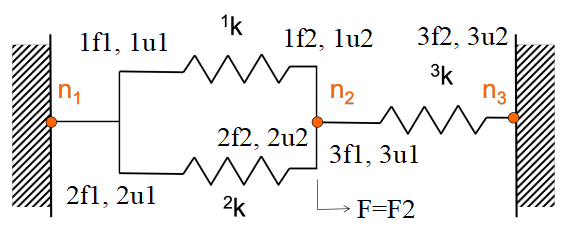
\includegraphics[width=0.5\textwidth]{figures/problem_1.png}
	\caption{Visualization of problem 1.}
	\label{fig:problem_1}
\end{figure}
Finally, the reaction forces can be calculated using the displacement $U_2$ as \begin{equation}
	F_1 = K_{12}\frac{F_2}{K_{22}} = -F_2\frac{{}^1k + {}^2k}{{}^1k + {}^2k + {}^3k}, \qquad F_3 = K_{32}\frac{F_2}{K_{22}} = -F_2\frac{{}^3k}{{}^1k + {}^2k + {}^3k}.
\end{equation}
}

\Que{How can an example of a static 2D discrete system be solved using the finite element method?}
\Ans{
Considering \cref{fig:problem_2}, the connectivity table can be set up as seen in \cref{tab:problem_2}.
\begin{figure}[h]
	\centering
	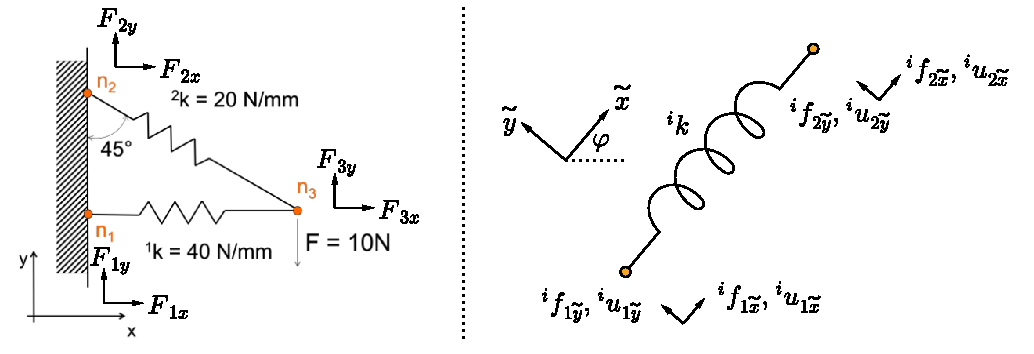
\includegraphics[width=0.8\textwidth]{figures/problem_2.pdf}
	\caption{Visualization of problem 2.}
	\label{fig:problem_2}
\end{figure}
Consider first of all the spring element drawn in the right panel of \cref{fig:problem_2}. In the reference frame $(\tilde{x},\tilde{y})$ of the spring element, one can set up the internal force equation as \begin{equation}
	{}^i\tilde{\vect{f}} = {}^i\tilde{\matr{k}}{}^i\tilde{\vect{u}} \quad \Leftrightarrow \quad \begin{pmatrix}
		{}^if_{1\tilde{x}} \\
		{}^if_{1\tilde{y}} \\
		{}^if_{2\tilde{x}} \\
		{}^if_{2\tilde{y}}
	\end{pmatrix} = \begin{pmatrix}
		{}^ik & 0 & -{}^ik & 0 \\
		0 & 0 & 0 & 0 \\
		-{}^ik & 0 & {}^ik & 0 \\
		0 & 0 & 0 & 0
	\end{pmatrix}\begin{pmatrix}
		{}^iu_{1\tilde{x}} \\
		{}^iu_{1\tilde{y}} \\
		{}^iu_{2\tilde{x}} \\
		{}^iu_{2\tilde{y}}
	\end{pmatrix}.
\end{equation} Using the rotation matrix (clockwise rotation about angle $\varphi$) \begin{equation}
	\matr{R} = \begin{pmatrix}
		\cos(\varphi) & \sin(\varphi) & 0 & 0 \\
		-\sin(\varphi) & \cos(\varphi) & 0 & 0 \\
		0 & 0 & \cos(\varphi) & \sin(\varphi)  \\
		0 & 0 & -\sin(\varphi) & \cos(\varphi) 
	\end{pmatrix},
\end{equation} one can relate ${}^i\tilde{\vect{f}}$ and ${}^i\tilde{\vect{u}}$ to their counterpart in the global reference frame $(x,y)$ as \begin{equation}
	{}^i\tilde{\vect{f}} = \matr{R} {}^i\vect{f}, \qquad {}^i\tilde{\vect{u}} = \matr{R} {}^i\vect{u}.
\end{equation} Using these equations, one can write \begin{equation}
	{}^i\vect{f} = \matr{R}^\top {}^i\tilde{\vect{f}} = \matr{R}^\top {}^i\tilde{\matr{k}} \matr{R}{}^i\vect{u} = {}^i\matr{k}{}^i\vect{u}
\end{equation} with ${}^i\matr{k} \doteq \matr{R}^\top {}^i\tilde{\matr{k}} \matr{R}$. Setting up now the connectivity table for the 2 nodes and 2 degrees of freedom for each node as shown in \cref{tab:problem_2}, one can construct the total global stiffness matrix $\matr{K}$ by means of ${}^1\matr{k}$ and ${}^2\matr{k}$. Defining the total global force vector $\vect{F} = (F_{1x}, F_{1y}, F_{2x}, F_{2y}, F_{3x}, F_{3y})^\top$ and the total global displacement vector as $\vect{U} = (U_{1x}, U_{1y}, U_{2x}, U_{2y}, U_{3x}, U_{3y})^\top$, we can write \begin{equation}
	\matr{K}\vect{U} = \vect{F}.
\end{equation} The boundary conditions are $F_{1x} = F_{1y} = F_{2x} = F_{2y} = F_{3x} = U_{1x} = U_{1y} = U_{2x} = U_{2y} = 0$, $F_{3y} = -\SI{10}{\newton}$ and $U_{3x}, U_{3y} \neq 0$. The problem is then solved by appropriate software tools. The solution of the problem is \begin{equation}
	\vect{F} = \begin{pmatrix}
		-10 \\
		0 \\
		10 \\
		10 \\
		0 \\
		-10
	\end{pmatrix} \,\si{\newton}, \qquad \vect{U} = \begin{pmatrix}
		0 \\
		0 \\
		0 \\
		0 \\
		0.25 \\
		-1.25
	\end{pmatrix}\,\si{\milli\meter}.
\end{equation}

\begin{table}
	\centering
	\begin{tabular}{|c|c|c|c|c|}
		\hline
		\text{Element} & n1, dof1 & n1, dof2 & n2, dof3 & n2, dof4 \\
		\hline\hline
		1 & 1 & 2 & 5 & 6 \\
		2 & 3 & 4 & 5 & 6 \\
		\hline
	\end{tabular}
	\caption{Connectivity table for the nodes of problem 2.}
	\label{tab:problem_2}
\end{table}	
}

\section{1D continuous system}
%\Que{How can a static 1D continuous system be solved using the finite element method?}
%\Ans{
%The finite element method is applied to a general one-dimensional boundary value problem where an unknown function \( u(x) \) is defined over the domain \( \Omega = [0, l] \) and governed by the differential equation  
%\begin{equation}
%\mathcal{L} u(x) = f(x), \quad x \in \Omega.
%\end{equation}
%The operator \( \mathcal{L} \) is a linear differential operator involving derivatives of \( u(x) \), and \( f(x) \) is a given source term. The function \( u(x) \) satisfies given boundary conditions. The weak formulation of this problem is obtained by multiplying the equation by a test function \( \delta u(x) \) and integrating over the domain, which leads to  
%\begin{equation}
%\int_{\Omega} \left[ \mathcal{L} u(x) - f(x) \right] \delta u(x) \,\mathrm{d}x = 0.
%\end{equation}
%Using integration by parts where necessary, this equation can be rewritten as  
%\begin{equation}
%\int_{\Omega} \bm{B} u(x) \delta u(x) \,\mathrm{d}x = \int_{\Omega} f(x) \delta u(x) \,\mathrm{d}x,
%\end{equation}
%where \( \bm{B} \) is a differential operator obtained after integration by parts.  
%
%The finite element discretization approximates \( u(x) \) using a piecewise function over a set of \( m \) elements that divide the domain \( \Omega \) into subdomains \( {}^e \Omega = [x_i, x_{i+1}] \). For each element \( e \), the function is approximated as  
%\begin{equation}
%{}^e u^h(x) = {}^e \bm{H}(x) \, {}^e \bm{q}.
%\end{equation}
%Here, \( {}^e \bm{H}(x) \) is the vector of shape functions, and \( {}^e \bm{q} \) is the vector of nodal unknowns associated with the element. The global approximation is obtained by assembling the local contributions from all elements, leading to  
%\begin{equation}
%u^h(x) = \sum_{e=1}^{m} {}^e \bm{H}(x) {}^e \boldsymbol{\mathbf{L}} \bm{q},
%\end{equation}
%where \( {}^e \boldsymbol{\mathbf{L}} \) is the localization matrix that maps local element values to the global system. The test function \( \delta u^h(x) \) follows the same structure.  
%
%The shape functions within each element are typically defined in a local coordinate system \( \xi \), for an element consisting of two nodes by  
%\begin{equation}
%{}^e h_1(\xi) = \frac{1}{2} (1 - \xi), \quad {}^e h_2(\xi) = \frac{1}{2} (1 + \xi)
%\end{equation} for example.
%The transformation between global and local coordinates is given by  
%\begin{equation}
%\xi(x) = \frac{2x - x_i - x_{i+1}}{ {}^e l }, \quad {}^e l = x_{i+1} - x_i.
%\end{equation}
%Expressed in terms of the global coordinate \( x \), the shape functions take the form  
%\begin{equation}
%{}^e h_1(x) = \frac{x_{i+1} - x}{x_{i+1} - x_i}, \quad {}^e h_2(x) = \frac{x - x_i}{x_{i+1} - x_i}.
%\end{equation}
%The global shape functions are obtained by assembling the shape functions from all elements.  
%
%Substituting the finite element approximation into the weak formulation results in the system of equations  
%\begin{equation}
%\sum_{e=1}^{m} \int_{{}^e \Omega} \bm{B} {}^e u^h(x) \delta u^h(x) \,\mathrm{d}x = \sum_{e=1}^{m} \int_{{}^e \Omega} f(x) \delta u^h(x) \,\mathrm{d}x.
%\end{equation}
%This leads to the linear system  
%\begin{equation}
%\boldsymbol{\mathbf{K}} \bm{q} = \bm{r},
%\end{equation}
%where the global stiffness matrix is obtained from the sum of element stiffness matrices  
%\begin{equation}
%{}^e \boldsymbol{\mathbf{K}} = \int_{{}^e \Omega} \bm{B}^T \boldsymbol{\mathbf{D}} \bm{B} \,\mathrm{d}x.
%\end{equation}
%The matrix \( \bm{B} \) is the derivative of the shape functions with respect to \( x \), and \( \boldsymbol{\mathbf{D}} \) is the material property matrix, which depends on the specific problem being solved. The global force vector is assembled from the local element force vectors  
%\begin{equation}
%{}^e \bm{r} = \int_{{}^e \Omega} f(x) {}^e \bm{H}^T \,\mathrm{d}x.
%\end{equation}
%For second-order differential equations such as elasticity or heat conduction, a typical form of the element stiffness matrix is  
%\begin{equation}
%{}^e \boldsymbol{\mathbf{K}} = \frac{1}{{}^e l} \begin{bmatrix} 1 & -1 \\ -1 & 1 \end{bmatrix},
%\end{equation}
%and the element force vector is given by  
%\begin{equation}
%{}^e \bm{r} = \int_{{}^e \Omega} f(x) {}^e \bm{H}^T \,\mathrm{d}x.
%\end{equation}
%
%The material property matrix \( \boldsymbol{\mathbf{D}} \) depends on the type of physical problem. In heat conduction, it is represented by the thermal conductivity \( k \). In linear elasticity, it is given by the product of Young’s modulus and the cross-sectional area, \( E A \), for one-dimensional problems. More generally, \( \boldsymbol{\mathbf{D}} \) contains the material properties governing the system's response. After assembling the global system and applying boundary conditions, the system is solved for \( \bm{q} \), providing an approximation of \( u(x) \) across the domain.  
%}

\Que{How does an example application of the static 1D continuous FEM method work?}
\Ans{
Consider a 1D problem of heat transfer given by the equation \begin{equation}
	q(x) = -k\frac{\mathrm{d}^2T(x)}{\mathrm{d}x^2},
\end{equation}
where $T(x)$ is the temperature at location $x$, $q(x)$ is a source function and $k$ is the thermal conductivity.

Let a particular problem be defined by the boundary conditions $T(0) = T(l) = 0$ and \begin{equation}
	q(x) = \begin{cases}
		q_0 & 0 \leq x \leq l/2 \\
		0 & l/2 < x \leq l
	\end{cases}.
\end{equation} Let $\delta T(x)$ be a weighting function, which satisfies the same boundary conditions as $T(x)$. The weak formulation of the differential equation with $\delta T(x)$ is then given by \begin{equation}\label{eq:weakform_prob_1}
	\int_{0}^l \left[k\frac{\mathrm{d}^2 T(x)}{\mathrm{d}x^2} + q(x)\right]\delta T(x)\,\mathrm{d}x \quad \forall \ \delta T(x).
\end{equation} By the partial integration rule \begin{equation}
	\int f(x) g^\prime (x)\,\mathrm{d}x = f(x)g(x) - \int f^\prime(x)g(x)\,\mathrm{d}x
\end{equation} and defining \begin{equation}
	f(x) \doteq k\delta T(x), \qquad g(x)\doteq \frac{\mathrm{d}T(x)}{\mathrm{d}x},
\end{equation} we obtain from \cref{eq:weakform_prob_1} the equation \begin{equation}
	\left[k\delta T(x)\frac{\mathrm{d}T(x)}{\mathrm{d}x}\right]_0^l - \int_{0}^l k\frac{\mathrm{d}T(x)}{\mathrm{d}x}\frac{\mathrm{d}\delta T(x)}{\mathrm{d}x}\,\mathrm{d}x = -\int_{0}^l q(x)\delta T(x)\,\mathrm{d}x = 0.
\end{equation} The first term vanishes, because we assume the same boundaries for $\delta T(x)$ as for $T(x)$, namely $\delta T(0) = \delta T(l) = 0$. Furthermore, the last integral can be simplified to \begin{equation}
	\int_{0}^l q(x)\delta T(x)\,\mathrm{d}x = q_0\int_{0}^{l/2}\delta T(x)\,\mathrm{d}x
\end{equation} due to the definition of $q(x)$. With that, we finally obtain \begin{equation}\label{eq:problem1}
	\int_{0}^l k\frac{\mathrm{d}T(x)}{\mathrm{d}x}\frac{\mathrm{d}\delta T(x)}{\mathrm{d}x}\,\mathrm{d}x = q_0\int_{0}^{l/2}\delta T(x)\,\mathrm{d}x \qquad \forall \ \delta T(x).
\end{equation}

Consider the finite element analysis task as depicted in \cref{fig:prob2}.
\begin{figure}[h]
	\centering
	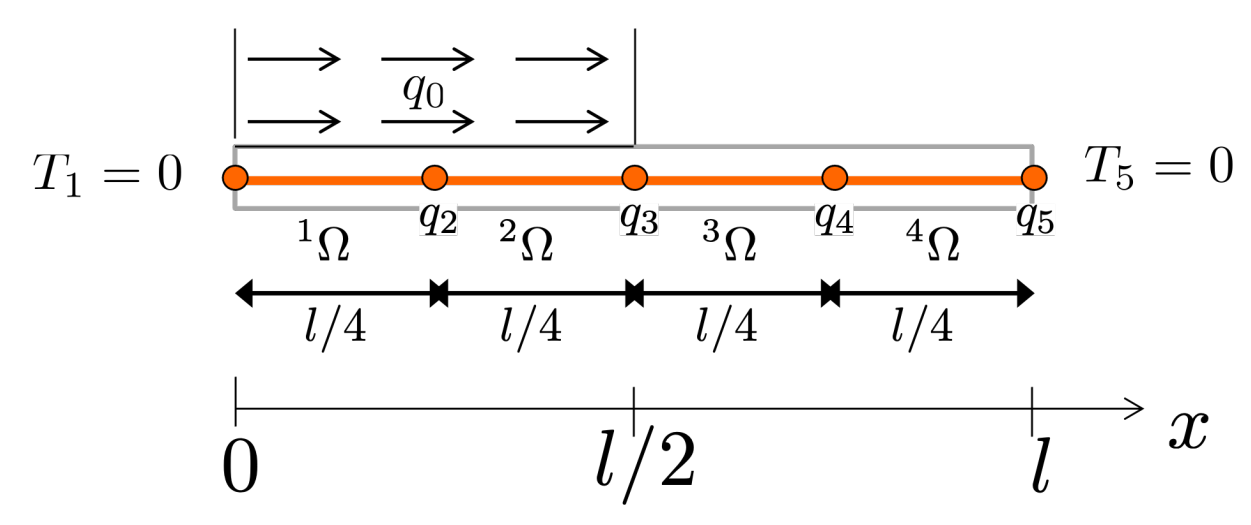
\includegraphics[width=0.5\textwidth]{figures/prob2.png}
	\caption{Visualization of problem 2.}
	\label{fig:prob2}
\end{figure}
Let now an individual element $^e\Omega$ be considered. The approximate solution $^eT^h(x)$ on this element shall be the sum of products between element shape functions and element unknowns; in vector form, this can be written as \begin{equation}
	^eT^h(x) = {} ^e\vect{H}(x) {}^e\vect{q},
\end{equation} where $^e\vect{H}(x) = ({}^eh_1(x), \dots , {}^eh_{^ep}(x))$ is a vector of element shape functions, where $^ep$ is the number of nodes for the element $e$. Furthermore, $^e\vect{q} = ({}^eq_1,\dots,{}^e q_{^ep})^\top$ is a vector of unknowns for each element $e$. The construction of the approximated solution on the complete space - not just on $^e\Omega$ - is achieved by assembling the element approximations. This requires a mapping between the global node numbering $\vect{q}$ and the local node vector $^e\vect{q}$. This is done by the localization matrix $^e\matr{L}$, which establishes the relation \begin{equation}
	^e\vect{q} ={} ^e\matr{L}\vect{q}, \qquad {}^eL_{ij} = \begin{cases}
		1, & \text{global node $j$ equal to local node $i$} \\
		0, & \text{otherwise}
	\end{cases}.
\end{equation} One can now write $T^h(x)$ and $\delta T^h(x)$ as 
\begin{align}
	\begin{aligned}
		T^h(x) = \sum_{e=1}^{m} {}^e T^h(x) = \sum_{e=1}^{m} {}^e\vect{H}(x) {}^e\vect{q} = \sum_{e=1}^{m} {}^e\vect{H}(x) {}^e\matr{L}\vect{q}
	\end{aligned}
\end{align} and \begin{equation}
	\delta T^h(x) = \sum_{e=1}^{m} {}^e \delta T^h(x) = \sum_{e=1}^{m} {}^e\vect{H}(x) {}^e\delta \vect{q} = \sum_{e=1}^{m} {}^e\vect{H}(x) {}^e\matr{L}\delta\vect{q}.
\end{equation}
Inserting this into \cref{eq:problem1} leads to \begin{equation}
	\sum_{e=1}^{m} \left[\int_{^e\Omega} k \frac{\mathrm{d}{}^e T^h(x)}{\mathrm{d}x}\frac{\mathrm{d}{}^e \delta T^h(x)}{\mathrm{d}x}\,\mathrm{d}x\right] = \sum_{e=1}^{m}\left[\int_{^e\Omega}{}^eq(x){}^e\delta T^h(x)\,\mathrm{d}x\right],
\end{equation} where $^eq(x)$ is the function $q(x)$ on each element. Using the defined equations and quantities, one obtains after several simplifications \begin{equation}
	\sum_{e=1}^{m}\delta \vect{q}^\top {}^e\matr{L}^\top \left[\int_{{}^e\Omega}k {}^e\vect{B}^\top {}^e\vect{B}\,\mathrm{d}x\right]{}^e\matr{L}\vect{q} = \sum_{e=1}^{m}\delta \vect{q}^\top {}^e\matr{L}^\top \left[\int_{{}^e\Omega}{} ^eq{}^e\vect{H}^\top\,\mathrm{d}x\right],
\end{equation} where ${}^e\vect{B} = \frac{\mathrm{d} {}^e\vect{H}}{\mathrm{d}x}$. Because the factor $\delta \vect{q}^\top$ is arbitrary and the same for both sides of the equation, it can be drawn out of the sum and subsequently left away, hence one obtains \begin{equation}
	\matr{K}\vect{q} = \vect{r}, \qquad \matr{K} = \sum_{e=1}^{m} {}^e\matr{L}^\top {}^e\matr{K} {}^e\matr{L}, \qquad \vect{r} = \sum_{e=1}^{m} {}^e\matr{L}^\top {}^e\vect{r},
\end{equation} where \begin{equation}
	{}^e\matr{K} = \int_{{}^e\Omega} k {}^e\vect{B}^\top {}^e\vect{B}\,\mathrm{d}x, \qquad {}^e\vect{r} = \int_{{}^e\Omega} {}^eq {}^e\vect{H}^\top \,\mathrm{d}x.
\end{equation}
An element ${}^e K_{ij}$ of the local stiffness matrix $^e\matr{K}$ is given by \begin{equation}\label{eq:int_K}
	{}^e K_{ij} = \int_{{}^e\Omega} k \frac{\mathrm{d}{}^e h_i(x)}{\mathrm{d}x}\frac{\mathrm{d}{}^e h_j(x)}{\mathrm{d}x}\,\mathrm{d}x,
\end{equation} and a component $^e r_i$ of the vector $^e\vect{r}$ is calculated as \begin{equation}\label{eq:int_r}
	^e r_i = \int_{{}^e\Omega} {}^e q(x) {}^e h_i(x)\,\mathrm{d}x.
\end{equation} In order to perform those integrals, the element shape functions $^e h_i(x)$ need to be defined. In the case of the problem at hand, the element shape functions are given according to \cref{fig:prob2_elem}.
\begin{figure}[h]
	\centering
	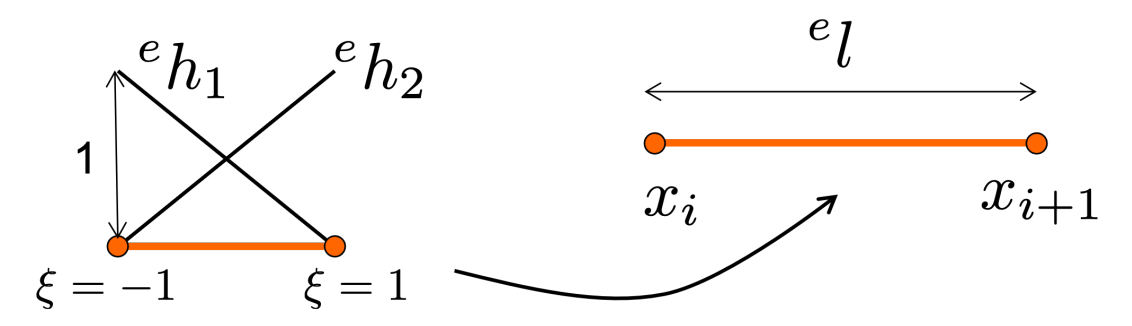
\includegraphics[width=0.4\textwidth]{figures/prob2_elem.png}
	\caption{Shape functions for one element in problem 2.}
	\label{fig:prob2_elem}
\end{figure} There are two nodes per element, hence there are two shape functions \begin{equation}
	^e h_1(\xi) = \frac{1}{2}(1-\xi), \qquad ^e h_2(\xi) = \frac{1}{2}(1 + \xi)
\end{equation} defined using the local coordinate $\xi$. These shape functions ensure, that the function $^eh_1$ is one at the first node and zero at the second node, and the opposite for $^e h_2$. The transformation $\xi \rightarrow x $ is given by the equation \begin{equation}
	\xi(x) = \frac{2x - x_i - x_{i+1}}{^e l}, \qquad {}^e l = x_{i+1} - x_i,
\end{equation} where $x_i$ denotes the global location of the global node $i$. Hence, $^e h_1(x)$ and $^e h_2(x)$ are given by \begin{equation}
	^e h_1(x) = \frac{x_{i+1}-x}{x_{i+1}-x_i}, \qquad {}^e h_2(x) = \frac{x-x_i}{x_{i+1}-x_i}.
\end{equation} With this, or using the chain rule as \begin{equation}
	\frac{\mathrm{d}{}^e h_i(\xi(x))}{\mathrm{d}x} = \frac{\partial {}^e h_i(\xi(x))}{\partial \xi}\frac{\mathrm{d} \xi(x)}{\mathrm{d}x}, \quad i \in \{1,2\},
\end{equation} the integrals \cref{eq:int_K} and \cref{eq:int_r} can be performed. In fact, we have \begin{align}
	^e K_{11} &= \int_{{}^e\Omega} k  \left(\frac{\partial {}^e h_1}{\partial \xi}\right)^2\left(\frac{\mathrm{d} \xi}{\mathrm{d}x}\right)^2\,\mathrm{d}x = \frac{k}{^e l} \int_{{}^e\Omega}\,\mathrm{d}x = \frac{k}{^el}\int_{-1}^{1} \frac{^e l}{2}\,\mathrm{d}\xi = \frac{k}{^e l}, \\
	^e K_{12}&= {}^e K_{21} = \int_{{}^e\Omega} k  \left(\frac{\partial {}^e h_1}{\partial \xi}\right)\left(\frac{\partial {}^e h_2}{\partial \xi}\right)\left(\frac{\mathrm{d} \xi}{\mathrm{d}x}\right)^2\,\mathrm{d}x = -\frac{k}{^e l} \int_{{}^e\Omega}\,\mathrm{d}x = -\frac{k}{^el}\int_{-1}^{1} \frac{^e l}{2}\,\mathrm{d}\xi = -\frac{k}{^e l}, \\
	^e K_{22} &= \int_{{}^e\Omega} k  \left(\frac{\partial {}^e h_2}{\partial \xi}\right)^2\left(\frac{\mathrm{d} \xi}{\mathrm{d}x}\right)^2\,\mathrm{d}x = \frac{k}{^e l} \int_{{}^e\Omega}\,\mathrm{d}x = \frac{k}{^el}\int_{-1}^{1} \frac{^e l}{2}\,\mathrm{d}\xi = \frac{k}{^e l}.
\end{align} Hence, the local stiffness matrix $^e \matr{K}$ is given by \begin{equation}
	^e \matr{K} = \frac{k}{^e l}\begin{pmatrix}
		1 & -1 \\
		-1 & 1
	\end{pmatrix}, \qquad ^e l = l/4.
\end{equation} Using $\matr{K} = \sum_{e=1}^{4}{}^e \matr{L}^\top {}^e \matr{K} {}^e\matr{L}$, one obtains the global stiffness matrix $\matr{K}$ as \begin{equation}
	\matr{K} = \frac{4k}{l}\begin{pmatrix}
		1 & -1 & 0 & 0 & 0 \\
		-1 & 2 & -1 & 0 & 0 \\
		0 & -1 & 2 & -1 & 0 \\
		0 & 0 & -1 & 2 & -1 \\
		0 & 0 & 0 & -1 & 1
	\end{pmatrix}.
\end{equation} Taking into account the information present in \cref{fig:prob2}, the components $^e r_i$ for $i \in\{1,2\}$ are similarly calculated as  
\begin{align}
	^1 r_1 &= \int_{{}^1\Omega} {}^1 q(x) {}^1 h_1(x)\,\mathrm{d}x = \frac{q_0}{2}\int_{0}^{l/4}\left(2-\frac{8x}{l}\right)\,\mathrm{d}x = \frac{q_0 l}{8}, \\
	^1 r_2 &= \int_{{}^1\Omega} {}^1 q(x) {}^1 h_2(x)\,\mathrm{d}x = \frac{q_0}{2}\int_{0}^{l/4}\left(\frac{8x}{l}\right)\,\mathrm{d}x = \frac{q_0 l}{8}, \\
	^2 r_1 &= \int_{{}^2\Omega} {}^2 q(x) {}^2 h_1(x)\,\mathrm{d}x = \frac{q_0}{2}\int_{l/4}^{l/2}\left(4-\frac{8x}{l}\right)\,\mathrm{d}x = \frac{q_0 l}{8}, \\
	^2 r_2 &= \int_{{}^2\Omega} {}^2 q(x) {}^2 h_2(x)\,\mathrm{d}x = \frac{q_0}{2}\int_{l/4}^{l/2}\left(-2+\frac{8x}{l}\right)\,\mathrm{d}x = \frac{q_0 l}{8}, \\
	^3 r_1 &= {}^3 r_2 = {}^4 r_1 = {}^4 r_2 = 0.
\end{align} Using $\vect{r} = \sum_{e=1}^{4} {}^e \matr{L}^\top {}^e\vect{r}$, the global vector $\vect{r}$ is given by \begin{equation}
	\vect{r} = \frac{q_0 l}{8}\begin{pmatrix}
		1 \\ 2 \\ 1 \\ 0  \\ 0
	\end{pmatrix}.
\end{equation} In total therefore, the system $\matr{K}\vect{q} = \vect{r}$ to be solved amounts to \begin{equation}
	\frac{k}{q_0l^2}\begin{pmatrix}
		32 & -32 & 0 & 0 & 0 \\
		-32 & 64 & -32 & 0 & 0 \\
		0 & -32 & 64 & -32 & 0 \\
		0 & 0 & -32 & 64 & -32 \\
		0 & 0 & 0 & -32 & 32
	\end{pmatrix}\begin{pmatrix}
		q_1 \\ q_2 \\ q_3 \\ q_4 \\ q_5
	\end{pmatrix} = \begin{pmatrix}
		1 \\ 2 \\ 1 \\ 0  \\ 0
	\end{pmatrix}.
\end{equation} Since the boundary conditions imply $q_1 = q_5 = 0$, we can leave away the first and last row and column of the problem; thus we need to solve 
\begin{equation}
	\frac{k}{q_0l^2}\begin{pmatrix}
		64 & -32 & 0 \\
		-32 & 64 & -32 \\
		0 & -32 & 64
	\end{pmatrix}\begin{pmatrix}
		q_2 \\ q_3 \\ q_4
	\end{pmatrix} = \begin{pmatrix}
		2 \\ 1 \\ 0
	\end{pmatrix}, 
\end{equation} from which the solution is obtained as \begin{equation}
	\begin{pmatrix}
		q_2 \\ q_3 \\ q_4
	\end{pmatrix} = \left[	\frac{k}{q_0l^2}\begin{pmatrix}
		64 & -32 & 0 \\
		-32 & 64 & -32 \\
		0 & -32 & 64
	\end{pmatrix}\right]^{-1}\begin{pmatrix}
		2 \\ 1 \\ 0
	\end{pmatrix}.
\end{equation}

The temperature $T(q_i)$ at node $i$ with $i \in \{1,2,\dots,5\}$ is then given by 
\begin{figure}[h]
	\centering
	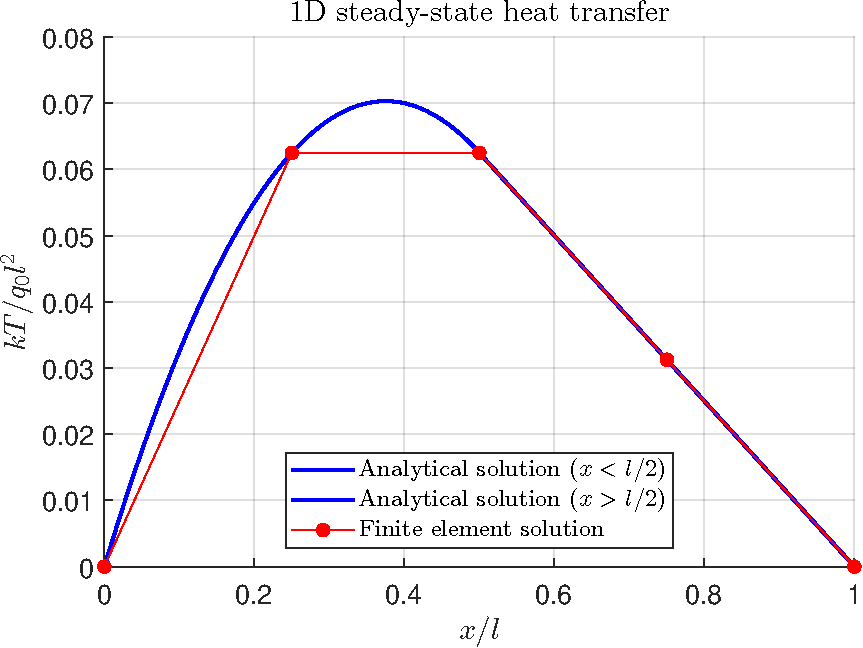
\includegraphics[width=0.5\textwidth]{figures/prob2_sol.pdf}
	\caption{Analytical and FEM solutions to problem 2 as depicted in \cref{fig:prob2}.}
	\label{fig:prob2_sol}
\end{figure}
means of $T(q_i) = q_i$. Using this and knowing the coordinates of node $i$ in the mesh, one obtains an approximate solution for the temperature (field) $T(x)$. The obtained solution for the developed finite element model (FEM) and the associated analytical solution to problem 2 are depicted in \cref{fig:prob2_sol}.
}

\section{2D continuous system}
%\Que{How can a static 2D continuous system be solved using the finite element method?}
%\Ans{Text.} % 

\Que{How does an example application of the static 2D continuous FEM method work?}
\Ans{
Consider the problem as seen in \cref{fig:step1}.
\begin{figure}[h]
	\centering
	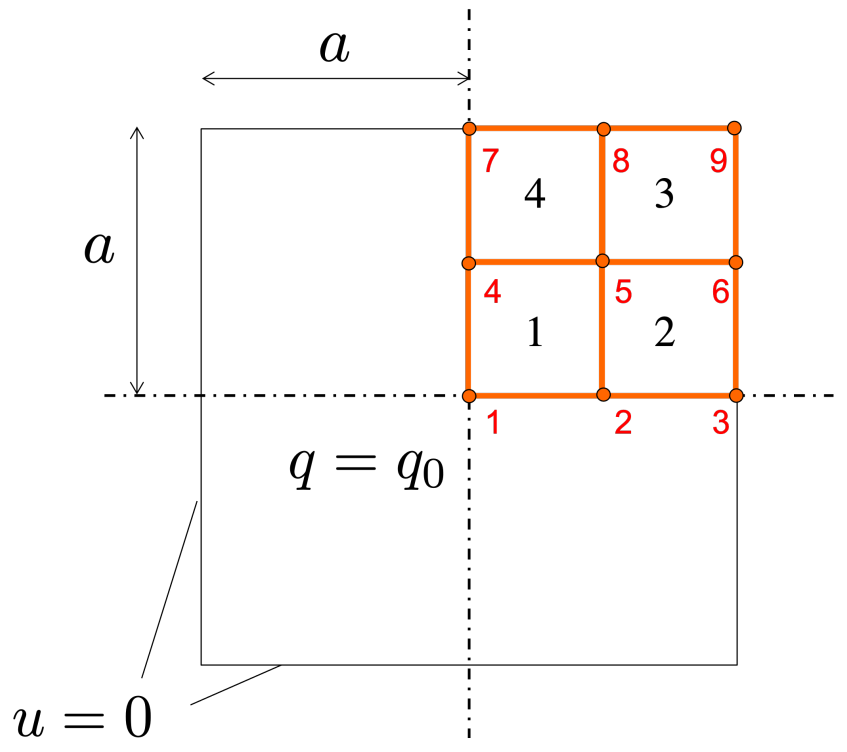
\includegraphics[width=0.5\textwidth]{figures/step1.png}
	\caption{Visualization of the problem to be solved using the finite element method.}
	\label{fig:step1}
\end{figure} The problem consists of a square plate with uniform conductivity $k$. There is a constant heat source $q(x,y) = q_0$ all over the plate, and the edges are held at constant temperature zero.

The governing equation for this problem is given by \begin{equation}\label{eq:strongform}
	k\vect{\nabla}^2 u(x,y) + q(x,y) = 0,
\end{equation} where it is assumed that the conductivity $k$ is uniform and constant over the domain of interest. Hereby, $u(x,y)$ is the temperature field to be approximated using the finite element method in 2D.

For this purpose, the weak form of the strong form \cref{eq:strongform} has to be derived first. The strategy is the same as in 1D; one multiplies the strong form equation by a weight function $\delta u(x,y)$ and integrates it over the domain $\Omega$ of interest:
\begin{equation}\label{eq:weakform}
	\int_{\Omega}\left[k\vect{\nabla}^2 u(x,y) + q(x,y)\right]\delta u(x,y)\,\mathrm{d}x\,\mathrm{d}y = 0, \qquad \forall \ \delta u(x,y).
\end{equation} This equation must be valid for any $\delta u(x,y)$ for it to be equivalent to the strong form \cref{eq:strongform} and thus to be a sound weak form of the problem. First of all, recall the Gauss theorem \begin{equation}
	\int_\Omega (\vect{\nabla}\cdot \vect{F})\,\mathrm{d}V_\Omega = \int_{\partial \Omega} \vect{F}\cdot \vect{n}_\Omega \,\mathrm{d}S_\Omega,
\end{equation} where $\Omega$ is the $m$-dimensional domain, $\partial\Omega$ is its boundary, $\mathrm{d}V_\Omega$ is the infinitesimal volume element of $\Omega$, $\mathrm{d}S_\Omega$ is the infinitesimal surface element of $\Omega$ and $\vect{n}_\Omega$ is a unit vector pointing everywhere perpendicularly outwards on $\partial \Omega$. Now, for some functions $f(x,y)$ and $g(x,y)$ we obtain $\vect{\nabla}(fg) = (\vect{\nabla}f)g + f(\vect{\nabla}g)$ by the product rule. Hence, we also obtain $f(\vect{\nabla}g) = \vect{\nabla}(fg) - (\vect{\nabla}f)g$. Defining $f \doteq \delta u$ and $g = k\vect{\nabla}u$, we thus get \begin{equation}
	\delta u k \vect{\nabla}^2 u = \vect{\nabla}\left(\delta u k\vect{\nabla}u\right) - (\vect{\nabla}\delta u) k \vect{\nabla}u.
\end{equation} Using this result and the Gauss theorem stated above, one can perform the simplifications \begin{align}
	\begin{aligned}
		0 &= \int_{\Omega}\left[k\vect{\nabla}^2 u + q\right]\delta u \,\mathrm{d}x\,\mathrm{d}y \\
		&= \int_\Omega \vect{\nabla}\left(\delta u k\vect{\nabla}u\right)\,\mathrm{d}x\,\mathrm{d}y -\int_\Omega k(\vect{\nabla}u)(\vect{\nabla}\delta u)\,\mathrm{d}x\,\mathrm{d}y + \int_\Omega q \delta u\,\mathrm{d}x\,\mathrm{d}y \\
		&= -\int_\Omega k(\vect{\nabla}u)(\vect{\nabla}\delta u)\,\mathrm{d}x\,\mathrm{d}y + \int_\Omega q \delta u\,\mathrm{d}x\,\mathrm{d}y,
	\end{aligned}
\end{align} where \begin{equation}
	\int_\Omega \vect{\nabla}\left(\delta u k\vect{\nabla}u\right)\, \mathrm{d}V_\Omega =\int_{\partial \Omega} (\delta u k\vect{\nabla}u) \cdot \vect{n}_\Omega \,\mathrm{d}S_\Omega = 0, \qquad \mathrm{d}V_\Omega = \mathrm{d}x\,\mathrm{d}y
\end{equation} because of the boundary condition $u(x,y) = 0$ and hence also $\delta u(x,y) = 0$ at the boundary $\partial \Omega$ of the domain $\Omega$. Exploiting the constant conductivity $k$ and the boundary condition $q(x,y) = q_0$ one obtains the weak form of the problem as \begin{equation}\label{eq:weakform1}
	k\int_{\Omega} \left[\vect{\nabla}u(x,y)\right]\left[\vect{\nabla}\delta u(x,y)\right]\,\mathrm{d}x\,\mathrm{d}y = q_0\int_\Omega \delta u(x,y)\,\mathrm{d}x\,\mathrm{d}y \qquad \forall \ \delta u(x,y).
\end{equation} Now, the function $u(x,y)$ is approximated by a sum of nodal constant unknowns $q_i$ and shape functions $h_i(x,y)$ multiplied by them, namely \begin{equation}\label{eq:discret_u}
	u(x,y) \approx u^h(x,y) = \sum_{i=1}^{p}h_i(x,y)q_i = \vect{H}(x,y)\vect{q},
\end{equation} where $\vect{H} = (h_1(x,y),\dots,h_p(x,y))$. Similarly, we have \begin{equation}\label{eq:discret_deltau}
	\delta u(x,y) \approx \delta u^h(x,y) = \sum_{i=1}^{p}h_i(x,y)\delta q_i = \vect{H}(x,y)\delta \vect{q},
\end{equation} where $\delta \vect{q} = (\delta q_1,\dots,\delta q_p)^\top$. Note that for a vector $\vect{b} = (b_1,\dots,b_p)$ and a constant vector $\vect{a} = (a_1,\dots,a_p)^\top$ it holds that \begin{equation}
	\vect{\nabla}(\vect{a}^\top \vect{b}^\top) = \vect{a}^\top (\vect{\nabla}\vect{b})^\top,
\end{equation} where $\vect{\nabla}\vect{b}$ is a $d \times p$ matrix, if $d$ is the dimensionality of the space, i.e. $\vect{\nabla} = (\partial_1,\dots,\partial_d)^\top$. Inserting now \cref{eq:discret_u} and \cref{eq:discret_deltau} into \cref{eq:weakform1} yields \begin{equation}
	\int_{\Omega} k\vect{\nabla}\left(\vect{H}\vect{q}\right)\vect{\nabla}\left(\vect{H} \delta \vect{q}\right)\,\mathrm{d}x\,\mathrm{d}y = \int_\Omega q_0 \vect{H}\delta \vect{q}\,\mathrm{d}x\,\mathrm{d}y.
\end{equation} Since $\vect{H}\vect{q}$ and $\vect{H}\delta \vect{q}$ are scalars, it holds that \begin{equation}
	\vect{H}\vect{q} = (\vect{H}\vect{q})^\top = \vect{q}^\top \vect{H}^\top, \qquad \vect{H}\delta \vect{q} = (\vect{H}\delta \vect{q})^\top = \delta \vect{q}^\top \vect{H}^\top
\end{equation} and furthermore \begin{equation}
	\vect{\nabla}(\vect{q}^\top \vect{H}^\top) = \vect{q}^\top (\vect{\nabla}\vect{H})^\top, \qquad \vect{\nabla}(\delta \vect{q}^\top \vect{H}^\top) = \delta \vect{q}^\top (\vect{\nabla}\vect{H})^\top, \qquad \vect{\nabla}(\vect{H}\vect{q}) = (\vect{\nabla}\vect{H})\vect{q}.
\end{equation} Therefore, we can rewrite the above equation as \begin{equation}
	\delta \vect{q}^\top \left[\int_\Omega k (\vect{\nabla}\vect{H})^\top (\vect{\nabla}\vect{H})\,\mathrm{d}x\,\mathrm{d}y\right] \vect{q} = \delta \vect{q}^\top \int_\Omega q_0 \vect{H}^\top \,\mathrm{d}x\,\mathrm{d}y.
\end{equation} Redefining $\vect{\nabla}\vect{H}\doteq \matr{B}$ and leaving away the constant factor $\delta \vect{q}^\top$ both on the right hand and left hand sides of the above equation yields \begin{equation}
	\underbrace{\left[\int_\Omega k \matr{B}^\top \matr{B}\,\mathrm{d}x\,\mathrm{d}y\right]}_{\doteq\,\matr{K}} \vect{q} = \underbrace{\int_\Omega q_0 \vect{H}^\top \,\mathrm{d}x\,\mathrm{d}y}_{\doteq\,\vect{r}} \quad \Leftrightarrow \quad \matr{K}\vect{q} = \vect{r}.
\end{equation} One can write the above equation also using local shape functions instead of global ones; then the above equation reads as \begin{equation}
	\underbrace{\left[\int_{{}^e \Omega} k {}^e \matr{B}(x,y)^\top {}^e \matr{B}(x,y)\,\mathrm{d}x\,\mathrm{d}y\right]}_{\doteq \, {}^e \matr{K}}  {}^e\vect{q} = \underbrace{\int_{{}^e \Omega} q(x,y) {}^e\vect{H}(x,y)^\top \,\mathrm{d}x\,\mathrm{d}y}_{\doteq \, {}^e\vect{r}}
\end{equation} with $\matr{K} = \sum_{e=1}^m {}^e \matr{L}^\top {}^e\matr{K}{}^e\matr{L}$ and $\vect{r} = \sum_{e=1}^m {}^e \matr{L}^\top {}^e \vect{r}$, where $m$ is the total element number in the discretized system and ${}^e \matr{L}$ is the localization matrix of element $e$ defined as \begin{equation}
	{}^e \vect{q} = {}^e \matr{L}\vect{q}, \qquad {}^e L_{ij} = \begin{cases}
		1, & \text{global node $j$ equal to local node $i$} \\
		0, & \text{otherwise}
	\end{cases}.
\end{equation}

Consider \cref{fig:shapefunct}. \begin{figure}[h]
	\centering
	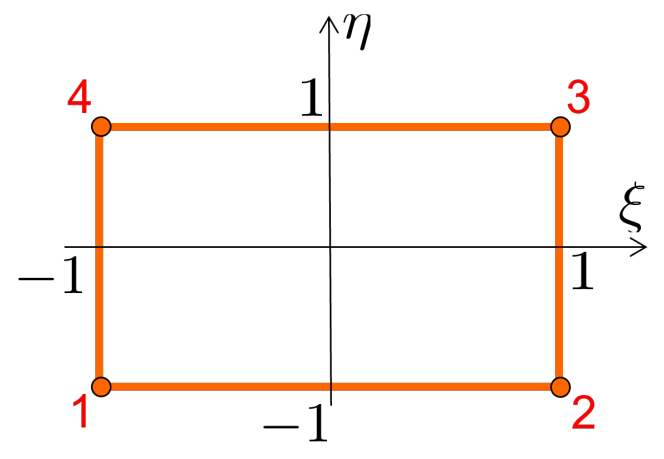
\includegraphics[width=0.3\textwidth]{figures/shapefunct.png}
	\caption{Local node numbering and coordinate system of a 2D rectangular finite element.}
	\label{fig:shapefunct}
\end{figure}
The local shape functions $ h_j(\xi,\eta)$ of such an element are given by \begin{align}\begin{aligned}
		h_1(\xi,\eta) &= \frac{1}{4}(1-\xi)(1-\eta), \qquad h_2(\xi,\eta) = \frac{1}{4}(1+\xi)(1-\eta), \\
		h_3(\xi,\eta) &= \frac{1}{4}(1+ \xi)(1+\eta), \qquad  h_4(\xi,\eta) = \frac{1}{4}(1-\xi)(1+\eta).
\end{aligned}\end{align} These shape functions each define a plane in 3D space, where $h_j(\xi,\eta)$ is one at node $j$ and zero at all the other nodes of the element. Now, the transformation ${}^e T$ of an element's coordinates to the global coordinates is given by \begin{equation}
	{}^e T : \mathbb{R}^2 \rightarrow \mathbb{R}^2, \begin{pmatrix} x \\ y
	\end{pmatrix} \mapsto \begin{pmatrix}
		{}^e x(\xi,\eta) = \sum_{i=1}^4 h_i(\xi,\eta)x_i \\
		{}^e y(\xi,\eta) = \sum_{i=1}^4 h_i(\xi,\eta)y_i
	\end{pmatrix}
\end{equation} where $x_i$ and $y_i$ denote the global coordinates of the local node $i$ of element $e$.

We now calculate ${}^1 T$ for the first element as shown in \cref{fig:step1}. We have \begin{equation}{}^1 T : \begin{pmatrix}
		x \\ y
	\end{pmatrix} \mapsto
	\begin{pmatrix}	{}^1 x(\xi,\eta) =  h_2(\xi,\eta)\frac{a}{2} + h_3(\xi,\eta)\frac{a}{2} = \frac{a}{4}(1+\xi) \\
		{}^1 y(\xi,\eta) = h_3(\xi,\eta)\frac{a}{2} + h_4(\xi,\eta)\frac{a}{2} = \frac{a}{4}(1+\eta)\end{pmatrix}.
\end{equation} Now, the Jacobian $\matr{J}_{{}^e T}$ of the transformation ${}^e T$ is given by \begin{equation}
	\matr{J}_{{}^e T} = \begin{pmatrix}
		\frac{\partial {}^e x}{\partial \xi} & \frac{\partial {}^e y}{\partial \xi} \\
		\frac{\partial {}^e x}{\partial \eta} & \frac{\partial {}^e y}{\partial \eta}\end{pmatrix}, \qquad \begin{pmatrix}
		\partial_\xi \\ \partial_\eta
	\end{pmatrix} = \begin{pmatrix}
		\frac{\partial {}^e x}{\partial \xi} & \frac{\partial {}^e y}{\partial \xi} \\
		\frac{\partial {}^e x}{\partial \eta} & \frac{\partial {}^e y}{\partial \eta}\end{pmatrix}\begin{pmatrix}
		\partial_x \\ \partial_y
	\end{pmatrix}= \matr{J}_{{}^e T}\begin{pmatrix}
		\partial_x \\ \partial_y
	\end{pmatrix}
\end{equation} and hence also \begin{equation}
	\begin{pmatrix}
		\partial_x \\ \partial_y
	\end{pmatrix} = \matr{J}_{{}^e T}^{-1} \begin{pmatrix}
		\partial_\xi \\ \partial_\eta
	\end{pmatrix}.
\end{equation} We have in particular \begin{equation}
	\frac{\partial {}^1 x}{\partial \xi} = \frac{a}{4}, \quad \frac{\partial {}^1 x}{\partial \eta} = 0, \quad \frac{\partial {}^1 y}{\partial \xi} = 0, \quad \frac{\partial {}^1 y}{\partial \eta} = \frac{a}{4}
\end{equation} and thus the Jacobian \begin{equation}
	\matr{J}_{{}^1 T} = \begin{pmatrix}
		\frac{a}{4} & 0 \\
		0 & \frac{a}{4}
	\end{pmatrix}, \qquad \matr{J}_{{}^1 T}^{-1} = \begin{pmatrix}
		\frac{4}{a} & 0 \\
		0 & \frac{4}{a}
	\end{pmatrix}, \qquad \det\left[\matr{J}_{{}^1 T}\right] = \frac{a^2}{16}.
\end{equation} Thus, the differential area element $\mathrm{d}x\,\mathrm{d}y$ transforms as $\mathrm{d}x\,\mathrm{d}y = \det\left[\matr{J}_{{}^e T}\right]\mathrm{d}\xi\,\mathrm{d}\eta$ for the coordinate transformation from global coordinates $(x,y)$ to the local coordinates $(\xi,\eta)$ of element $e$.

Now, the B-matrix ${}^e \matr{B}$ is defined as \begin{equation}
	\vect{\nabla}{}^e\vect{H} = \begin{pmatrix}
		\partial_x \\ \partial_y
	\end{pmatrix} (h_1(x,y),\dots,h_4(x,y)) = \begin{pmatrix}
		\partial_x {}^e h_1 & \partial_x{}^e  h_2 & \partial_x{}^e  h_3 & \partial_x {}^e h_4 \\
		\partial_y {}^e h_1 & \partial_y{}^e  h_2 & \partial_y{}^e  h_3 & \partial_y {}^e h_4
	\end{pmatrix},
\end{equation} where the notation ${}^a h_i = h_i(\xi,\eta)$ and ${}^e h_i = h_i(x,y)$ was adopted. We can further write \begin{equation}
	\partial_x {}^e h_i = \frac{\partial {}^a h_i}{\partial \xi}\frac{\partial \xi}{\partial x} + \frac{\partial {}^a h_i}{\partial \eta}\frac{\partial \eta}{\partial x}, \qquad \partial_y {}^e h_i = \frac{\partial {}^a h_i}{\partial \xi}\frac{\partial \xi}{\partial y} + \frac{\partial {}^a h_i}{\partial \eta}\frac{\partial \eta}{\partial y}.
\end{equation} For the element $e=1$, the derivatives are $\partial_x \xi = \frac{4}{a}$, $\partial_x \eta = 0$, $\partial_y \xi = 0$ and $\partial_y \eta = \frac{4}{a}$. Calculating furthermore \begin{equation}
	\begin{matrix}
		\frac{\partial {}^a h_1}{\partial \xi} =& -\frac{1}{4}(1-\eta) \\
		\frac{\partial {}^a h_2}{\partial \xi} =& \frac{1}{4}(1-\eta) \\
		\frac{\partial {}^a h_3}{\partial \xi} =& \frac{1}{4}(1+\eta) \\
		\frac{\partial {}^a h_4}{\partial \xi} =& -\frac{1}{4}(1+\eta)
	\end{matrix} \qquad  \qquad
	\begin{matrix}
		\frac{\partial {}^a h_1}{\partial \eta} =& -\frac{1}{4}(1-\xi) \\
		\frac{\partial {}^a h_2}{\partial \eta} =& -\frac{1}{4}(1+\xi) \\
		\frac{\partial {}^a h_3}{\partial \eta} =& \frac{1}{4}(1+\xi) \\
		\frac{\partial {}^a h_4}{\partial \eta} =& \frac{1}{4}(1-\xi)
	\end{matrix}
\end{equation} one can assemble the B-matrix in local coordinates as \begin{equation}
	{}^a \matr{B} = \frac{1}{a}\begin{pmatrix}
		-(1-\eta) & (1-\eta) & (1 + \eta) & - (1+\eta) \\
		-(1-\xi) & -(1+\xi) & (1 + \xi) & (1 - \xi)
	\end{pmatrix}.
\end{equation}

Recall, that the element stiffness matrix ${}^e \matr{K}$ for the problem at hand is given as \begin{equation}
	{}^e \matr{K} = \int_{{}^e \Omega} k {}^e\matr{B}^\top {}^e \matr{B}\,\mathrm{d}x\,\mathrm{d}y = \int_{{}^a\Omega} k {}^a \matr{B}^\top {}^a\matr{B} \det\left[\matr{J}_{{}^e T}\right]\,\mathrm{d}\xi\,\mathrm{d}\eta.
\end{equation}
For a product of matrices $\matr{X}\matr{Y}$ the entry $[\matr{X}\matr{Y}]_{ij}$ is given by $[\matr{X}\matr{Y}]_{ij} = \sum_k X_{ik}Y_{kj}$. Considering the element $e=1=a$, we calculate now the elements ${}^1 K_{11}$ and ${}^1 K_{13}$. The former element is calculated as \begin{align}
	\begin{aligned}
		{}^1 K_{11} &= \int_{{}^a\Omega}k \left[{}^a \matr{B}^\top {}^a\matr{B}\right]_{11}\det\left[\matr{J}_{{}^1 T}\right]\,\mathrm{d}\xi\,\mathrm{d}\eta = \frac{ka^2}{16}\int_{\xi=-1}^{1}\int_{\eta=-1}^{1}\left[{}^a \matr{B}^\top {}^a\matr{B}\right]_{11}\,\mathrm{d}\xi\,\mathrm{d}\eta \\
		&= \frac{ka^2}{16}\int_{\xi=-1}^{1}\int_{\eta=-1}^{1}\left[\sum_{k=1}^{2} {}^a B_{k1} {}^a B_{k1}\right]\,\mathrm{d}\xi\,\mathrm{d}\eta = \frac{ka^2}{16}\int_{\xi=-1}^{1}\int_{\eta=-1}^{1}\left[{}^a B_{11}^2 + {}^a B_{21}^2\right]\,\mathrm{d}\xi\,\mathrm{d}\eta \\
		&= \frac{ka^2}{16}\int_{\xi=-1}^{1}\int_{\eta=-1}^{1}\left[\frac{1}{a^2}(1-\eta)^2 + \frac{1}{a^2}(1-\xi)^2\right]\,\mathrm{d}\xi\,\mathrm{d}\eta \\
		&= \frac{k}{16}\int_{\eta=-1}^{1}\left(\frac{14}{3}-4\eta + 2\eta^2\right)\,\mathrm{d}\eta = \frac{2k}{3}.
	\end{aligned}
\end{align} The element ${}^1 K_{13}$ is then calculated as \begin{align}
	\begin{aligned}
		{}^1 K_{13} &= \int_{{}^a\Omega}k \left[{}^a \matr{B}^\top {}^a\matr{B}\right]_{13}\det\left[\matr{J}_{{}^1 T}\right]\,\mathrm{d}\xi\,\mathrm{d}\eta = \frac{ka^2}{16}\int_{\xi=-1}^{1}\int_{\eta=-1}^{1}\left[{}^a \matr{B}^\top {}^a\matr{B}\right]_{13}\,\mathrm{d}\xi\,\mathrm{d}\eta \\
		&= \frac{ka^2}{16}\int_{\xi=-1}^{1}\int_{\eta=-1}^{1}\left[\sum_{k=1}^{2} {}^a B_{k1} {}^a B_{k3}\right]\,\mathrm{d}\xi\,\mathrm{d}\eta \\ &= -\frac{k}{16}\int_{\xi=-1}^{1}\int_{\eta=-1}^{1}\left[(1-\eta)(1+\eta)+(1-\xi)(1+\xi)\right]\,\mathrm{d}\xi\,\mathrm{d}\eta = -\frac{k}{3}.
	\end{aligned}
\end{align} Calculating all the elements of ${}^1 \matr{K}$ in the same way one obtains \begin{equation}
	{}^1 \matr{K} = \frac{k}{6}\begin{pmatrix}
		4 & -1 & -2 & -1 \\
		-1 & 4 & -1 & -2 \\
		-2 & -1 & 4 & -1 \\
		-1 & -2 & -1 & 4
	\end{pmatrix}.
\end{equation} One can see that the formerly calculated elements ${}^1 K_{11}$ and ${}^1 K_{13}$ coincide with the elements in that matrix.

Recall from above, that the element load vector is defined as \begin{equation}
	{}^e \vect{r} = \int_{{}^e \Omega} q(x,y) {}^e\vect{H}(x,y)^\top \,\mathrm{d}x\,\mathrm{d}y = \int_{{}^a\Omega} {}^a q(\xi,\eta) {}^a\vect{H}(\xi,\eta)^\top \det\left[\matr{J}_{{}^e T}\right] \,\mathrm{d}\xi\,\mathrm{d}\eta.
\end{equation} The vector ${}^ a \vect{H}(\xi,\eta)$ is given by \begin{equation}
	{}^a\vect{H}(\xi,\eta)^\top = \frac{1}{4}\begin{pmatrix}
		(1-\xi)(1-\eta) \\
		(1+\xi)(1-\eta) \\
		(1+\xi)(1+\eta) \\
		(1-\xi)(1+\eta)
	\end{pmatrix}.
\end{equation} for the element $e=1=a$. Hence, the component ${}^1 r_2$ of the load vector ${}^1 \vect{r}$ is calculated as \begin{align}
	\begin{aligned}
		{}^1 r_2 &= \frac{q_0a^2}{64}\int_{{}^a\Omega}  (1+\xi)(1-\eta)\,\mathrm{d}\xi\,\mathrm{d}\eta = \frac{q_0a^2}{64}\int_{\eta=-1}^1 \int_{\xi=-1}^{1}  (1+\xi)(1-\eta)\,\mathrm{d}\xi\,\mathrm{d}\eta \\
		&= \frac{q_0 a^2}{64}\int_{\xi=-1}^1 (2+2\xi)\,\mathrm{d}\xi = \frac{q_0a^2}{16}.
	\end{aligned}
\end{align} Calculating all the other components ${}^1 r_i$ for $i \in \{1,2,3,4\}$ one arrives at the element load vector \begin{equation}
	{}^1\vect{r} = \frac{q_0 a^2}{16}(1,1,1,1)^\top.
\end{equation}

Now, the global load vector $\vect{r}$ will have nine components, as there are nine global nodes. In order to assemble the global load vector, we build a connectivity table:
\begin{table}[h!]
	\centering
	\begin{tabular}{|c|c|c|c|c|}
		\hline
		\textbf{Element} & \textbf{GN for LN1} & \textbf{GN for LN2} & \textbf{GN for LN3} & \textbf{GN for LN4} \\
		\hline\hline
		1 & 1 & 2 & 5 & 4 \\
		\hline
		2 & 2 & 3 & 6 & 5 \\
		\hline
		3 & 5 & 6 & 9 & 8 \\
		\hline
		4 & 4 & 5 & 8 & 7 \\
		\hline
	\end{tabular}
	\caption{Connectivity table the heat transfer problem as visualized in \cref{fig:step1}. The table shows the global node (GN) associated to local nodes (LN).}
	\label{tab:connectivity_table}
\end{table}
Based on this connectivity table, one can now build the global load vector $\vect{r}$ as \begin{equation}
	\vect{r} = \frac{q_0a^2}{16}\begin{pmatrix}
		1 \\
		1+1 \\
		1 \\
		1+1\\
		1+1+1+1 \\
		1+1 \\
		1 \\
		1+1 \\
		1
	\end{pmatrix} = \frac{q_0a^2}{16}\begin{pmatrix}
		1 \\ 2 \\ 1 \\ 2 \\ 4 \\ 2 \\ 1 \\ 2 \\ 1
	\end{pmatrix}.
\end{equation}

Using Gauss integration, one can approximate the integral to calculate the element stiffness matrix ${}^e \matr{K}$ and element load vector ${}^e \vect{r}$ as \begin{align}\begin{aligned}
		{}^e \matr{K}& = \int_{{}^a\Omega} k {}^a \matr{B}^\top(\xi,\eta) {}^a \matr{B}(\xi,\eta) \det\left[\matr{J}_{{}^e T}(\xi,\eta)\right]\,\mathrm{d}\xi\,\mathrm{d}\eta \\
		&\approx \sum_{j=1}^{s}\omega(j){}^a\matr{B}^\top[\xi(j),\eta(j)]  {}^a\matr{B}[\xi(j),\eta(j)] \det\left(\matr{J}_{{}^e T}[\xi(j),\eta(j)]\right)
\end{aligned}\end{align} and
\begin{align}
	\begin{aligned}
		{}^e \vect{r} &= \int_{{}^a\Omega} {}^a q(\xi,\eta) {}^a\vect{H}^\top(\xi,\eta) \det\left[\matr{J}_{{}^e T}(\xi,\eta)\right]\,\mathrm{d}\xi\,\mathrm{d}\eta \\
		&\approx \sum_{j=1}^{s}\omega(j){}^aq\left[\xi(j),\eta(j)\right]{}^a\vect{H}^\top [\xi(j),\eta(j)] \det\left(\matr{J}_{{}^e T}[\xi(j),\eta(j)]\right),
	\end{aligned}
\end{align} where $\omega(j)$, $\xi(j)$ and $\eta(j)$ are the weights and element coordinate values at the integration point $j \in\{1,\dots,s\}$ for each element. What is now needed in order to implement the calculations is expressing the B-matrix, the H-vector and the Jacobian in terms of local coordinates $(\xi(j),\eta(j))$ at the integration points. Furthermore, the weights $\omega(j)$ need to be known for a chosen geometry. For using one or four integration points per element, the weights are given as seen in \cref{fig:weights}.
\begin{figure}[h]
	\centering
	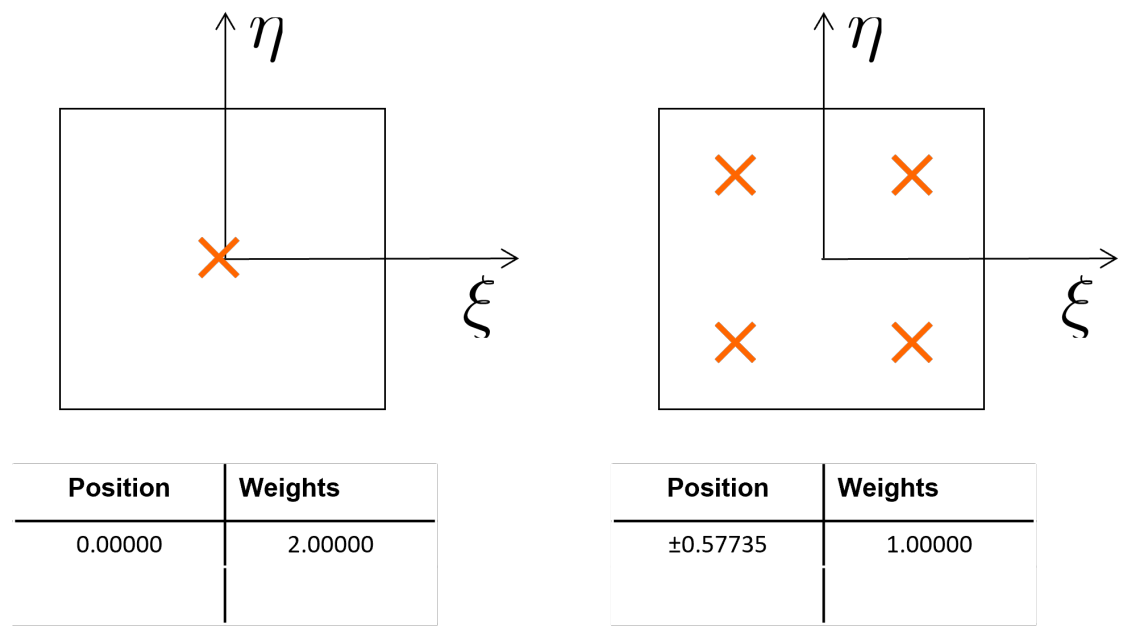
\includegraphics[width=0.5\textwidth]{figures/weights.png}
	\caption{Weights for using one or four integration points for a 2D-rectangular element.}
	\label{fig:weights}
\end{figure}

The coordinate transformation ${}^e T$ can be written in matrix form as \begin{equation}
	[x(\xi,\eta),y(\xi,\eta)] = [h_1(\xi,\eta),\dots,h_p(\xi,\eta)]\begin{pmatrix}
		{}^e x_1  & {}^e y_1 \\
		\vdots & \vdots \\
		{}^e x_p & {}^e y_p
	\end{pmatrix} = {}^a \vect{H}(\xi,\eta)({}^e \vect{x}, {}^e \vect{y}),
\end{equation} where ${}^e \vect{x}$ and ${}^e \vect{y}$ are the coordinates of the $p$ nodes of element $e$ in the global coordinate system. The Jacobian $\matr{J}_{{}^e T}(\xi,\eta)$ can then be calculated as \begin{align}\begin{aligned}
		\matr{J}_{{}^e T}(\xi,\eta) &= \begin{pmatrix}
			\frac{\partial {}^e x(\xi,\eta)}{\partial \xi} & \frac{\partial {}^e y(\xi,\eta)}{\partial \xi}\\
			\frac{\partial {}^e x(\xi,\eta)}{\partial \eta} & \frac{\partial {}^e y(\xi,\eta)}{\partial \eta}
		\end{pmatrix} = \begin{pmatrix}
			\partial_\xi \\ \partial_\eta
		\end{pmatrix} [x(\xi,\eta), y(\xi,\eta)] =  \begin{pmatrix}
			\partial_\xi \\ \partial_\eta
		\end{pmatrix}{}^a \vect{H}(\xi,\eta)({}^e \vect{x}, {}^e \vect{y}) \\
		&= \underbrace{\begin{pmatrix}
				\frac{\partial h_1(\xi,\eta)}{\partial \xi},\dots,\frac{\partial h_p(\xi,\eta)}{\partial \xi} \\
				\frac{\partial h_1(\xi,\eta)}{\partial \eta},\dots,\frac{\partial h_p(\xi,\eta)}{\partial \eta}
		\end{pmatrix}}_{\doteq \,\matr{A}(\xi,\eta)}({}^e \vect{x}, {}^e \vect{y}) = {}^a\matr{A}(\xi,\eta)({}^e \vect{x}, {}^e \vect{y}).
\end{aligned}\end{align} The B-matrix ${}^a\matr{B}(\xi,\eta)$ can be calculated as \begin{align}\begin{aligned}
		{}^a\matr{B}(\xi,\eta) &= \begin{pmatrix}
			\partial_x \\ \partial_y
		\end{pmatrix} {}^e\vect{H}(x,y) =  \matr{J}_{{}^e T}^{-1}\begin{pmatrix}
			\partial_\xi \\ \partial_\eta
		\end{pmatrix}{}^a \vect{H}(\xi,\eta) = \matr{J}_{{}^e T}^{-1} \begin{pmatrix}
			\frac{\partial h_1(\xi,\eta)}{\partial \xi},\dots,\frac{\partial h_p(\xi,\eta)}{\partial \xi} \\
			\frac{\partial h_1(\xi,\eta)}{\partial \eta},\dots,\frac{\partial h_p(\xi,\eta)}{\partial \eta}
		\end{pmatrix} \\
		&= \matr{J}_{{}^e T}^{-1}{}^a \matr{A}(\xi,\eta).
\end{aligned}\end{align} With these results and the weights from \cref{fig:weights}, one can now calculate the finite element model using Gauss integration for $s=1$ or $s=4$ integration points per element. The results obtained by Gauss integration are visualized in \cref{fig:distribution}.
\begin{figure}[h]
	\centering
	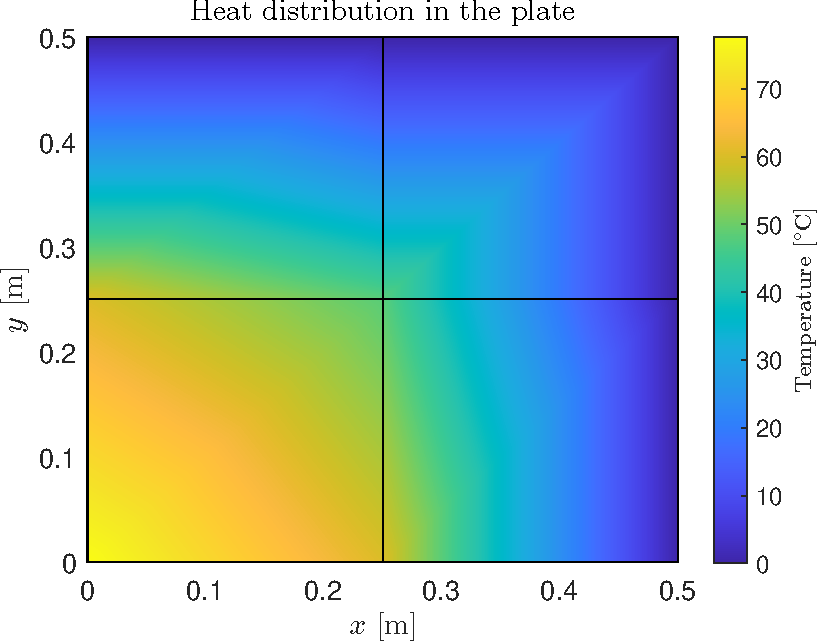
\includegraphics[width=0.5\textwidth]{figures/distribution.pdf}
	\caption{Solution obtained by Gauss integration for the heat conduction problem.}
	\label{fig:distribution}
\end{figure}
} 

\Que{What is the principle of Gauss integration (Gauss quadrature) used in finite element solvers?}
\Ans{
The principle of Gauss integration - also known as Gauss quadrature - is based on approximating an integral using optimally chosen integration points and corresponding weights. In general, one would like to evaluate an integral of the form
\begin{equation}
	I = \int_{-1}^{1} f(x) \,\mathrm{d}x \approx \sum_{i=1}^{n}w_if(x_i).
\end{equation} Now, consider that $f(x)$ may be approximated very well using a polynomial $p_{2n-1}(x)$ of degree $2n-1$, where $n \in \mathbb{N}$. This is possible for almost all smooth functions, given sufficiently high order $n$. Now, Gauss integration relies on intelligently and carefully choosing the integration points $x_i$ and weights $w_i$ and is thus yields exact results for polynomials up to degree $2n-1$ using $n$ integration points $x_i$ and correspondingly $n$ weights $w_i$. 

Consider now the space of polynomials with the basis $\{1, x, x^2, x^3, \dots\}$ and the inner product defined as \begin{equation}
	\langle p, q \rangle = \int_{-1}^1 p(x)q(x)\,\mathrm{d}x.
\end{equation} The so-called Legendre polynomials $L_n(x)$ are obtained by the Gram-Schmidt orthogonalization procedure as a basis of the space of polynomials, hence the Legendre polynomials up to and including order $n$ form a basis of space of polynomials up to $n$'th order and are thus equivalent to the basis $\{1, x, x^2, x^3, \dots\}$. But the Legendre polynomials have the property \begin{equation}
\langle L_i, L_j\rangle = \int_{-1}^{1}L_i(x)L_j(x)\,\mathrm{d}x = 0, \qquad i \neq j
\end{equation} by the orthogonal property of Legendre polynomials. This also means, that the Legendre polynomial $L_n(x)$ is orthogonal to any polynomial $p_{n-1}(x)$ of order $n-1$, namely \begin{equation}
\langle L_n, p_{n-1}\rangle = \int_{-1}^{1} L_n(x)p_{n-1}(x)\,\mathrm{d}x=0.
\end{equation}

At this point it is important to realize, that any polynomial $p_{2n-1}(x)$ of order $2n-1$ can be written in the form \begin{equation}
	p_{2n-1}(x) = q_{n-1}(x)L_n(x) + r_{n-1}(x),
\end{equation} where $q_{n-1}(x)$ and $r_{n-1}(x)$ are polynomials up to order $n-1$. This follows from polynomial division \begin{equation}
\frac{p_{2n-1}(x)}{L_n(x)} = q_{n-1}(x) + \frac{r_{n-1}(x)}{L_n(x)}.
\end{equation} Calculating now the integral for $p_{2n-1}(x)$ yields \begin{equation}
\int_{-1}^{1}p_{2n-1}(x)\,\mathrm{d}x = \int_{-1}^{1}q_{n-1}(x)L_n(x)\,\mathrm{d}x + \int_{-1}^{1} r_{n-1}(x)\,\mathrm{d}x = \int_{-1}^{1} r_{n-1}(x)\,\mathrm{d}x,
\end{equation} where the first term has vanished because of the orthogonality property of the Legendre polynomial $L_n(x)$ with any other polynomial of maximal degree $n-1$. Another important property of Legendre polynomials is, that the each Legendre polynomial $L_n(x)$ has exactly $n$ roots and all of these roots lie in the interval $[-1,1]$. Recalling the goal to find optimal weights $w_i$ and evaluation points $x_i$ to approximate the integral $I = \int_{-1}^{1} f(x) \,dx \approx \sum_{i=1}^{n}w_if(x_i)$. Now, choosing the roots $x_1,\dots,x_n$ of the Legendre polynomial $L_n(x)$ as evaluation points for the polynomial $p_{2n-1}(x)$, we have the situation \begin{equation}
\sum_{i=1}^n w_ip_{2n-1}(x_i) = \sum_{i=1}^n w_i q_{n-1}(x_i)L_n(x_i) + \sum_{i=1}^n w_i r_{n-1}(x_i) = \sum_{i=1}^n w_i r_{n-1}(x_i),
\end{equation} because $L_n(x_i) = 0$ for all $i \in \{1,\dots,n\}$. Now, one can choose the weights $w_i$ in such a way, that \begin{equation}
\int_{-1}^1 p_{2n-1}(x)\,\mathrm{d}x = \sum_{i=1}^n w_ip_{2n-1}(x_i) = \sum_{i=1}w_ir_{n-1}(x_i) = \int_{-1}^{1}r_{n-1}(x)\,\mathrm{d}x
\end{equation} holds exactly. This is done by solving the linear system of equations \begin{equation}\label{eq:vandermode_equation}
\begin{pmatrix}
	1 & 1 & \dots & 1 \\
	x_1 & x_2 & \dots & x_n \\
	x_1^2 & x_2^2 & \dots & x_n^2 \\
	\vdots & \vdots & \ddots & \vdots \\
	x_1^{n-1} & x_2^{n-1} & \dots & x_n^{n-1}
\end{pmatrix}\begin{pmatrix}
w_1 \\ w_2 \\ \vdots \\ w_n
\end{pmatrix} = \begin{pmatrix}
\int_{-1}^{1} 1 \,\mathrm{d}x \\
\int_{-1}^{1} x \,\mathrm{d}x \\
\int_{-1}^{1} x^2 \,\mathrm{d}x \\
\vdots \\
\int_{-1}^{1} x^{n-1} \,\mathrm{d}x
\end{pmatrix}
\end{equation} The $n$ weights obtained in such a way ensure, that all powers of $x$ up to order $n-1$ are integrated exactly over the interval $[-1,1]$ by the sum $\sum_{i=1}^n w_i x_i^{k}$ for $k \in \{0, 1, \dots, n-1\}$. Recall, that the $x_i$ are the roots of the $n$'th Legendre polynomial. That is to say, choosing the weights as described ensures \begin{equation}
\int_{-1}^{1} x^k\,\mathrm{d}x = \sum_{i=1}^n w_i x_i^k, \qquad k \leq n-1.
\end{equation} Writhing the polynomial $r_{n-1}(x)$ as \begin{equation}
r_{n-1}(x) = c_{n-1} x^{n-1} + c_{n-1} x^{n-2} + \dots + c_{1}x^1 + c_0 = \sum_{j=0}^{n-1} c_j x^j
\end{equation} therefore yields \begin{align}
\begin{aligned}
	\int_{-1}^{1}r_{n-1}(x)\,\mathrm{d}x &= \int_{-1}^{1}\sum_{j=1}^{n-1}c_jx^j\,\mathrm{d}x = \sum_{j=0}^{n-1}c_j\int_{-1}^{1}x^j\,\mathrm{d}x = \sum_{j=0}^{n-1}c_j\sum_{i=1}^{n}w_ix_i^j = \sum_{i=1}^{n}w_i\sum_{j=0}^{n-1}c_jx_i^j  \\ &= \sum_{i=1}^{n}w_i r_{n-1}(x_i).
\end{aligned}
\end{align} Putting everything together we have \begin{equation}
\int_{-1}^1 p_{2n-1}(x)\,\mathrm{d}x = \sum_{i=1}^{n}w_ip_{2n-1}(x_i),
\end{equation} if the weights $w_i$ are obtained by solving \cref{eq:vandermode_equation} and if the $x_i$ are the roots of the $n$'th Legendre polynomial $L_n(x)$.

Recall now that the initial goal was to calculate $I=\int_{-1}^{1}f(x)\,\mathrm{d}x$ by a weighted sum $\sum_{i=1}^{n}w_if(x_i)$. Let for the following material $w_i$ always be the weights obtained by solving \cref{eq:vandermode_equation} and $x_i$ the roots of the $n$'th degree Legendre polynomial $L_n(x)$. Now if $f(x)$ is identical to a polynomial of degree $2n-1$, we have $f(x) = p_{2n-1}(x)$ and thus by the above result \begin{equation}
	\int_{-1}^{1}f(x)\,\mathrm{d}x = \sum_{i=1}^{n}w_i f(x_i).
\end{equation} If $f(x)$ is not identical, but very similar to a polynomial of degree $2n-1$, we have $f(x) \approx p_{2n-1}(x)$ and hence the approximate result \begin{equation}
\int_{-1}^{1}f(x)\,\mathrm{d}x \approx \sum_{i=1}^{n}w_if(x_i)
\end{equation} holds. Note, that the

As an example, we consider the procedure for $n=3$, allowing for exact integration of polynomials up to order $2n-1 = 5$ using Gauss integration. For this, we need the Legendre polynomial $L_3(x)$ and its roots given by \begin{equation}
	L_3(x) = \frac{1}{2}\left(5x^3 - 3x\right), \qquad  x_1=-\sqrt{3/5},\ x_2 = 0, \ x_3 = \sqrt{3/5}.
\end{equation} Now, \cref{eq:vandermode_equation} yields the system of equations \begin{equation}
\begin{pmatrix}
	1 & 1 & 1 \\
	-\sqrt{\nicefrac{3}{5}} & 0 & \sqrt{\nicefrac{3}{5}} \\
	\nicefrac{3}{5}  & 0 & \nicefrac{3}{5}
\end{pmatrix}\begin{pmatrix}
w_1 \\ w_2 \\ w_3
\end{pmatrix} = \begin{pmatrix}
2 \\ 0 \\ \nicefrac{2}{3}
\end{pmatrix}
\end{equation} to be solved. Solving this yields $w_1 = 0.55555556$, $w_2 = 0.88888889$, $w_3= 0.55555556$. Given this scheme, one can integrate functions $f(x)$ that are well approximated by a fifth order polynomial extremely well; much better and faster than with the trapezoidal rule for example.

Two remarks remain to be made: First, if one has a general interval $[a,b]$ to integrate over, namely $\int_{a}^{b}f(x)\,\mathrm{d}x$, one can simply use change of variables formula \begin{equation}
 \int_{a}^{b}f(x)\,\mathrm{d}x = \int_{y(a)}^{y(b)}f(x(y))\frac{\mathrm{d}x(y)}{\mathrm{d}y}\,\mathrm{d}y.
\end{equation} In our case we use $y(x) = \frac{2x-(a+b)}{b-a}$ leading to \begin{equation}
\int_{a}^{b}f(x)\,\mathrm{d}x = \frac{b-a}{2}\int_{-1}^{1}f\left(\frac{b-a}{2}y+ \frac{a+b}{2}\right)\,\mathrm{d}y.
\end{equation} As a second remark it shall be noted, that the Legendre polynomials can be calculated recursively as \begin{equation}
L_0(x) = 1, \quad L_1(x) = x, \quad L_{n+1}(x) = \frac{(2n+1)L_n(x) - nL_{n-1}(x)}{n+1}
\end{equation} and the weights used for Gauss integration can be found directly via the formula \begin{equation}
w_i = \frac{2}{(1-x_i^2)\left[L_n^\prime(x_i)\right]^2},
\end{equation} where $x_i$ is the $i$'th root of $L_n(x)$ and $L_n^\prime(x)$ is the derivative of $L_n(x)$ with respect to $x$.
}

\section{3D continuous system}
%\Que{How can a static 3D continuous system be solved using the finite element method?}
%\Ans{
%Text.
%}
\Que{How does an example application of the static 3D continuous FEM method work?}
\Ans{
The finite element method for static problems in 3D works exactly analogous to the 2D method, with the difference that the finite elements are now in 3D rather than in 3D. This makes a slight reshaping of the H-vector containing the element shape functions necessary. Furthermore, the transformation $T$ from global coordinates $\vect{x} = (x,y,z)^\top$ to element coordinates $\vect{\xi} = (\xi,\eta,\zeta)^\top$ is given
The transformation from element coordinates $\vect{\xi}$ to global coordinates by \begin{equation}
	{}^e T:\vect{x} = \vect{x}(\vect{\xi}) = \sum_{i=1}^{{}^e p} {}^e h_i(\vect{\xi}){}^e \vect{x}_i = {}^e \matr{H}(\vect{\xi}) {}^e \vect{x},
\end{equation} where ${}^e \vect{x}$ is defined as \begin{equation}
	{}^e \vect{x} = ({}^e x_{1}, {}^e y_{1}, {}^e z_{1}, \dots, {}^e x_{{}^e p}, {}^e y_{{}^e p}, {}^e z_{{}^e p})
\end{equation} and ${}^e \matr{H}(\vect{x})$ is given by \begin{align}\small\begin{aligned}
		{}^e \matr{H}(\vect{x}) &= ({}^e \matr{H}_1(\vect{x}),\dots,{}^e \matr{H}_{{}^e p}(\vect{x}))
		\\
		 &= \begin{pmatrix}
			{}^e h_1(\vect{x}) & 0 & 0 & {}^e h_2(\vect{x}) & 0 & 0 & \hdots & {}^e h_{{}^e p}(\vect{x}) & 0 & 0 \\
			0 & {}^e h_1(\vect{x}) & 0 & 0 & {}^e h_2(\vect{x}) & 0 & \hdots & 0 & {}^e h_{{}^e p}(\vect{x}) & 0 \\
			0 & 0 & {}^e h_1(\vect{x}) & 0 & 0 & {}^e h_2(\vect{x}) & \hdots & 0 & 0 & {}^e h_{{}^e p}(\vect{x})
		\end{pmatrix}.
\end{aligned}\end{align} 

The function $\vect{u}(\vect{x})$ to find by the finite element method is given by the approximation $\vect{u}(\vect{x}) \approx \vect{u}^h(\vect{x})$. The approximated solution $\vect{u}^h(\vect{x})$ can be further decomposed into element solutions ${}^e \vect{u}^h(\vect{x})$ by means of \begin{equation}
	\vect{u}^h(\vect{x}) = \sum_{e=1}^{m}{}^e \vect{u}^h(\vect{x}),
\end{equation} where $m \in \mathbb{N}$ is the number of elements in the FEM system. The element solutions ${}^e\vect{u}^h(\vect{x})$ are approximated by the sum of element shape functions ${}^e h_i(\vect{x})$ multiplied by the nodal unknowns ${}^e \vect{q}_i$ for all nodes $i \in \{1,\dots,{}^e p\}$ with ${}^e p \in \mathbb{N}$ the number of nodes for element $e$. That is, we have \begin{equation}
{}^e \vect{u}^h(\vect{x}) = \sum_{i=1}^{{}^e p}{}^e h_i(\vect{x}){}^e\vect{q}_i = \sum_{i=1}^{{}^e p} {}^e \matr{H}_i(\vect{x}) {}^e \vect{q}_i = {}^e \matr{H}(\vect{x}){}^e \vect{q},
\end{equation} where ${}^e \vect{q} = ({}^e \vect{q}_1, \dots, {}^e \vect{q}_{{}^e p})^\top$.
}

\section{General continuous and time-dependent systems}
\Que{How can an example of a general case of a time-dependent partial differential equation (PDE) be solved using the finite element method?}
\Ans{
Let us consider a one-dimensional, time- and space-dependent boundary value problem governed by the partial differential equation (PDE)
\begin{equation}
	\frac{\partial u(x,t)}{\partial t} - \frac{\partial}{\partial x}\left(k(x)\frac{\partial u(x,t)}{\partial x}\right) = f(x,t), \quad x \in [0,L] = \Omega, \quad t > 0
\end{equation} subject to Dirichlet boundary conditions \begin{equation}
u(0,t) = u_{x0}, \quad u(L, t) = u_{xL}, \quad t > 0, \quad u(x,0) = u_{t0}(x),
\end{equation} where the last equation is an initial condition rather than a boundary condition. This is the strong form of the problem. In order to obtain a numerical solution to the PDE, we must convert it to the weak form. This is done by multiplying both sides of the PDE with weighting function $\delta u(x,t)$ and integrating over the domain $\Omega$ as \begin{equation}
\int_\Omega \frac{\partial u(x,t)}{\partial t}\delta u(x,t)\,\mathrm{d}x - \int_\Omega \frac{\partial}{\partial x}\left(k(x)\frac{\partial u(x,t)}{\partial x}\right)\delta u(x,t)\,\mathrm{d}x = \int_\Omega f(x,t)\delta u(x,t)\,\mathrm{d}x.
\end{equation} where we require the weighting function (variation) $\delta u(x,t)$ to be zero at the boundary of the integration domain $\Omega$. In order for the above weak form to be equivalent to the strong form, the formulation must hold for any weighting function $\delta u(x,t)$. Using integration by parts of the second term in the above weak form formulation and exploiting that the weighting function $\delta u(x,t)$ goes to zero at integration boundaries, we obtain \begin{equation}\label{eq:weakformgeneral}
\int_\Omega \frac{\partial u(x,t)}{\partial t}\delta u(x,t)\,\mathrm{d}x + \int_\Omega k(x)\frac{\partial u(x,t)}{\partial x}\frac{\partial \delta u(x,t)}{\partial x}\,\mathrm{d}x = \int_\Omega f(x,t)\delta u(x,t)\,\mathrm{d}x.
\end{equation} Now, let the function $u(x,t)$ be approximated by a hypothesis function $u^h(x,t)$, such that $u(x,t) \approx u^h(x,t)$. The hypothesis function shall be defined element-wise as \begin{equation}
u^h(x,t) = \sum_{e=1}^{m}{}^e u^h(x,t),
\end{equation} where the element-wise function ${}^e u^h(x,t)$ shall be given as the product of the element shape functions ${}^e h_i(x)$ and the nodal unknowns ${}^e q_i(t)$ as \begin{equation}\label{eq:hypothesisfunctions}
{}^e u^h(x,t) = \sum_{i=1}^{{}^e p}{}^e h_i(x){}^e q_i(t) = {}^e \vect{H}(x){}^e \vect{q}(t), \quad {}^e \delta u^h(x,t) = \sum_{i=1}^{{}^e p}{}^e h_i(x){}^e \delta q_i(t) = {}^e \vect{H}(x){}^e \delta \vect{q}(t)
\end{equation} where ${}^e \vect{H}(x) = ({}^e h_1(x),\dots,{}^e h_{{}^e p}(x))^\top$ with ${}^e p$ being the number of nodes per element $e$ and ${}^e \vect{q}(t) = ({}^e q_1(t),\dots,{}^e q_{{}^e p}(t))^\top$. Also the weighting function $\delta u(x,t)$ is approximated in the same way using the element shape functions and nodal unknowns, as shown above. The connection of the element system to the global system is established via the localization matrix ${}^e \matr{L}$ given by a connectivity table such that \begin{equation}
{}^e \vect{q} = {}^e \matr{L} \vect{q},
\end{equation} which means that we have \begin{align}
\begin{aligned}
	u^h(x,t) &= \sum_{e=1}^{m}{}^e u^h(x,t) = \sum_{e=1}^{m}{}^e\vect{H}(x){}^e \vect{q} = \sum_{e=1}^{m}{}^e \vect{H}(x){}^e \matr{L} \vect{q}, \\
	\delta u^h(x,t) &= \sum_{e=1}^{m}{}^e u^h(x,t) = \sum_{e=1}^{m}{}^e\vect{H}(x){}^e \delta\vect{q} = \sum_{e=1}^{m}{}^e \vect{H}(x){}^e \matr{L} \delta \vect{q}.
\end{aligned}
\end{align} 
One can also define the system on global scale, not with element-wise defined shape functions. In this case, we have just \begin{equation}\label{eq:hypothesisfunctionsglobal}
	u^h(x,t) = \vect{H}(x)\vect{q}(t), \quad \delta u^h(x,t) = \vect{H}(x)\delta\vect{q}(t),
\end{equation} where $\vect{H}(x) = (h_1(x),\dots,h_n(x))$ now contains all shape functions for the whole system, also defined on the whole domain $\Omega$; and $\vect{q}(t) = (q_1(t),\dots,q_n(t))^\top$ contains all $n$ nodal unknowns of the system. Inserting \cref{eq:hypothesisfunctionsglobal} into \cref{eq:weakformgeneral} leads after some simplifications to \begin{equation}
\int_{\Omega} \vect{H}(x)^\top \vect{H}(x)\,\mathrm{d}x \cdot \frac{\mathrm{d} \vect{q}(t)}{\mathrm{d} t} + \int_\Omega k(x)\frac{\mathrm{d}\vect{H}(x)^\top}{\mathrm{d}x}\frac{\mathrm{d}\vect{H}(x)}{\mathrm{d}x}\,\mathrm{d}x\cdot \vect{q}(t) = \int_\Omega f(x,t)\vect{H}(x)^\top \,\mathrm{d}x.
\end{equation} Defining the mass matrix $\matr{M}$, the stiffness matrix $\matr{K}$ and the load vector $\vect{r}(t)$ as \begin{align}\small\begin{aligned}
\matr{M} \doteq \int_{\Omega} \vect{H}(x)^\top \vect{H}(x)\,\mathrm{d}x, \quad \matr{K} \doteq \int_\Omega k(x)\frac{\mathrm{d}\vect{H}(x)^\top}{\mathrm{d}x}\frac{\mathrm{d}\vect{H}(x)}{\mathrm{d}x}\,\mathrm{d}x,\quad \vect{r}(t)\doteq \int_\Omega f(x,t)\vect{H}(x)^\top \,\mathrm{d}x, 
\end{aligned}\end{align} we can write the system to be solved as \begin{equation}\label{eq:globalsystem}
\matr{M}\frac{\mathrm{d}\vect{q}(t)}{\mathrm{d}t} + \matr{K}\vect{q}(t) = \vect{r}(t).
\end{equation} One can also express everything element-wise as \begin{equation}
\matr{M} = \sum_{e=1}^m {}^e \matr{L}^\top {}^e \matr{M} {}^e \matr{L}, \quad \matr{K} = \sum_{e=1}^m {}^e \matr{L}^\top {}^e \matr{K} {}^e \matr{L}, \quad \vect{r}(t) = \sum_{e=1}^{m}{}^e \matr{L}^\top {}^e \vect{r}(t).
\end{equation} and 
\begin{align}\footnotesize\begin{aligned}
		{}^e \matr{M} \doteq \int_{{}^e\Omega} {}^e\vect{H}(x)^\top {}^e\vect{H}(x)\,\mathrm{d}x, \quad {}^e\matr{K} \doteq \int_{{}^e\Omega} k(x)\frac{\mathrm{d}{}^e\vect{H}(x)^\top}{\mathrm{d}x}\frac{\mathrm{d}{}^e\vect{H}(x)}{\mathrm{d}x}\,\mathrm{d}x,\quad {}^e\vect{r}(t)\doteq \int_{{}^e\Omega} f(x,t){}^e\vect{H}(x)^\top \,\mathrm{d}x.
\end{aligned}\end{align}
Now, once one has assembled the global system \cref{eq:globalsystem}, it needs to be solved by application of the boundary and initial conditions. Now, the initial condition $\vect{q}(t=0)$ is given by $u(x,t=0) = u_{t0}(x)$, which is specified. Hence, time integration of the system \cref{eq:globalsystem} is necessary. There are several ways to do this, where the most straightforward methods are the explicit and implicit Euler methods.

Both methods start with approximating the derivative $\frac{\mathrm{d}\vect{q}(t)}{\mathrm{d}t}$ as \begin{equation}
	\frac{\mathrm{d}\vect{q}(t)}{\mathrm{d}t}\Biggr|_{t=j\Delta t} \approx \frac{\vect{q}^{j+1}-\vect{q}^{j}}{\Delta t}
\end{equation} by discretizing $\vect{q}(t)$ into discrete timesteps $\Delta t$, where $\vect{q}^j = \vect{q}(t^j) =\vect{q}(j\Delta t)$ and $\vect{r}^j = \vect{r}(t^j) = \vect{r}(j\Delta t)$. Now, the explicit Euler method approximates the differential equation \cref{eq:globalsystem} by \begin{equation}\label{eq:explicitintegration}
\matr{M}\frac{\vect{q}^{j+1}-\vect{q}^{j}}{\Delta t} + \matr{K}\vect{q}^j = \vect{r}^j,
\end{equation} whereas the implicit method approximates it as 
\begin{equation}
\label{eq:implicitintegration}
\matr{M}\frac{\vect{q}^{j+1}-\vect{q}^{j}}{\Delta t} + \matr{K}\vect{q}^{j+1} = \vect{r}^{j+1}.
\end{equation} The implicit formulation ensures that stiffness and mass effects are treated at the future time $t^{j+1}$, leading to better stability as compared to the explicit method. However, the implicit method requires solving a linear system of equations at each timestep, whereas the explicit method provides a simple equation to compute at each timestep. That is, the explicit method \cref{eq:explicitintegration} is rearranged to \begin{equation}
\vect{q}^{j+1} = \vect{q}^j + \Delta t \matr{M}^{-1}\left(\vect{r}^j - \matr{K}\vect{q}^j\right),
\end{equation} whereas the implicit method \cref{eq:implicitintegration} amounts to \begin{equation}
\left(\matr{M} + \Delta t \matr{K}\right)\vect{q}^{j+1} = \matr{M}\vect{q}^j + \Delta t \vect{r}^{j+1}.
\end{equation}
}

\Que{How can as simple FEM example with time integration be calculated?}
\Ans{
Consider the 1D heat equation, which is of the form \begin{equation}
	\frac{\partial T(x,t)}{\partial t} - \frac{\partial}{\partial x}\left(k(x)\frac{\partial T(x,t)}{\partial x}\right) = f(x,t).
\end{equation} We assume $f(x,t) = 0$ and use the boundary and initial conditions \begin{equation}
T(x=0,t) = \SI{0}{\kelvin}, \quad T(x = L, t) = \SI{0}{\kelvin}, \quad T(x, t=0) = T_0 \sin(\pi x)
\end{equation} with $T_0 = \SI{1}{\kelvin}$ and $L = \SI{1}{\meter}$. The thermal conductivity is furthermore assumed to be constant $k(x) = k = \SI{1}{\watt\meter^{-1}\kelvin^{-1}}$. We set the number of nodes $n=7$ and hence the number of elements to $m=6$ and use linear elements with two nodes and the shape functions \begin{equation}
{}^e h_1(\xi) = \frac{1}{2}(1-\xi), \qquad {}^e h_2(\xi) = \frac{1}{2}(1+\xi).\end{equation} Following the treatment outlined above, with ${}^e \vect{H}(x) = ({}^e h_1(x), {}^e h_2(x))$ the element mass matrix ${}^e \matr{M}$ is given by \begin{equation}
{}^e \matr{M} = \int_{{}^e \Omega} {}^e\vect{H}(x)^\top {}^e \vect{H}(x)\,\mathrm{d}x = \int_{-1}^{1}{}^e\vect{H}(x(\xi))^\top {}^e \vect{H}(x(\xi))\left|\frac{\mathrm{d}x(\xi)}{\mathrm{d}\xi}\right|\,\mathrm{d}\xi,
\end{equation} the element stiffenss matrix ${}^e \matr{K}$ by \begin{equation}
{}^e \matr{K} = \int_{{}^e\Omega}k\frac{\mathrm{d}{}^e \vect{H}(x)^\top}{\mathrm{d}x}\frac{\mathrm{d}{}^e \vect{H}(x)}{\mathrm{d}x}\,\mathrm{d}x = \int_{-1}^{1} k\frac{\mathrm{d}{}^e \vect{H}(x(\xi))^\top}{\mathrm{d}\xi}\frac{\mathrm{d}{}^e \vect{H}(x(\xi))}{\mathrm{d}\xi}\left(\frac{\mathrm{d}\xi(x)}{\mathrm{d}x}\right)^2\left|\frac{\mathrm{d}x(\xi)}{\mathrm{d}\xi}\right|\,\mathrm{d}\xi
\end{equation} and the element load vector ${}^e \vect{r}(t)$ as \begin{equation}
{}^e \vect{r}(t) = \int_{{}^e \Omega} f(x,t){}^e\vect{H}(x)\top\,\mathrm{d}x = \int_{-1}^{1}0\cdot {}^e \vect{H}(x(\xi))\left|\frac{\mathrm{d}x(\xi)}{\mathrm{d}\xi}\right|\,\mathrm{d}\xi .
\end{equation} These quantities are calculated to be \begin{equation}
{}^e \matr{M} = \frac{L}{32}\begin{pmatrix}
	2 & 1 \\ 1 & 2
\end{pmatrix}, \qquad {}^e \matr{K} = \frac{6k}{L}\begin{pmatrix}
1 & -1 \\ -1 & 1
\end{pmatrix}, \qquad {}^e \vect{r}(t) = \begin{pmatrix}
 0 \\ 0
\end{pmatrix}.
\end{equation} The assembled quantities are furthermore given by \begin{align}\scriptsize\begin{aligned}
\mathbf{M} = \frac{L}{32}
\begin{pmatrix}
	2 & 1 & 0 & 0 & 0 & 0 & 0 \\
	1 & 4 & 1 & 0 & 0 & 0 & 0 \\
	0 & 1 & 4 & 1 & 0 & 0 & 0 \\
	0 & 0 & 1 & 4 & 1 & 0 & 0 \\
	0 & 0 & 0 & 1 & 4 & 1 & 0 \\
	0 & 0 & 0 & 0 & 1 & 4 & 1 \\
	0 & 0 & 0 & 0 & 0 & 1 & 2
\end{pmatrix}, \quad \mathbf{K} = \frac{6k}{L}
\begin{pmatrix}
1 & -1 & 0 & 0 & 0 & 0 & 0 \\
-1 & 2 & -1 & 0 & 0 & 0 & 0 \\
0 & -1 & 2 & -1 & 0 & 0 & 0 \\
0 & 0 & -1 & 2 & -1 & 0 & 0 \\
0 & 0 & 0 & -1 & 2 & -1 & 0 \\
0 & 0 & 0 & 0 & -1 & 2 & -1 \\
0 & 0 & 0 & 0 & 0 & -1 & 1
\end{pmatrix},\quad \mathbf{r}(t) = \begin{pmatrix} 0 \\ 0 \\ 0 \\ 0 \\ 0 \\ 0 \\ 0 \end{pmatrix}.
\end{aligned}\end{align} Now, the nodal unknowns $\vect{q}(t) = (q_1(t),\dots,q_7(t))^\top$ are calculated using the explicit Euler method. The initial condition is given by sampling from $T(x, t=0) = T_0\sin(\pi x)$ at the locations $x_1,\dots,x_7$ of the seven nodes. 
\begin{figure}[h]
	\centering
	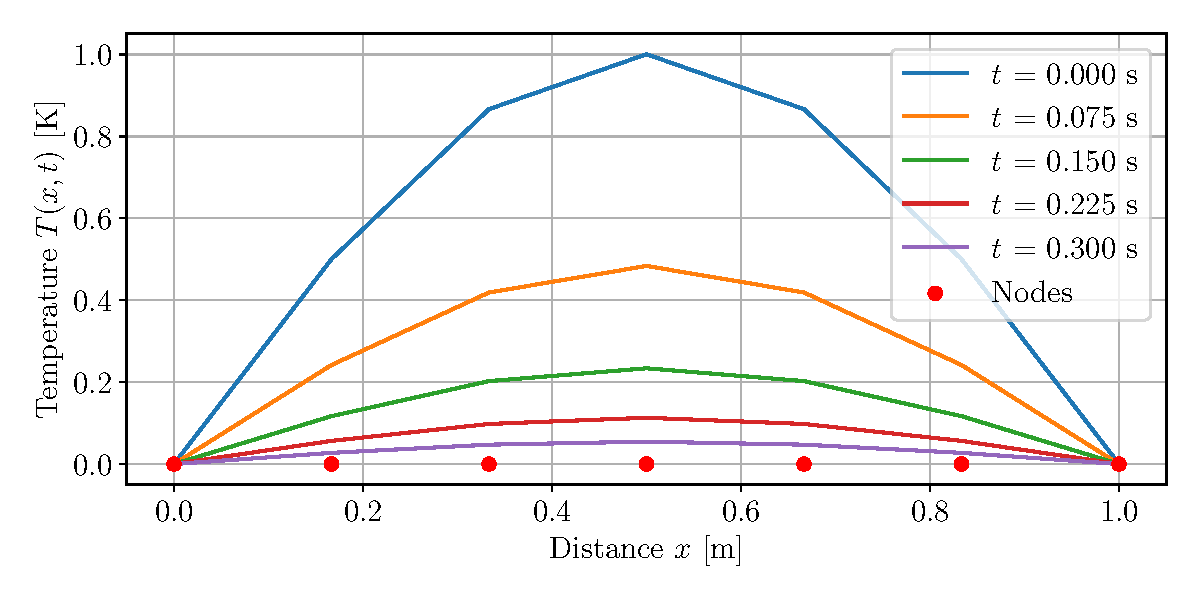
\includegraphics[width=0.6\textwidth]{figures/resultexampletimeint.pdf}
	\caption{Result for the presented example.}
	\label{fig:resultexampletimeint}
\end{figure}
This leads to the nodal unknowns vector $\vect{q}^0$ at time $t=0$. Using the explicit Euler method, each time iteration step is now given by \begin{equation}
\vect{q}^{j+1} = \vect{q}^j + \Delta t \matr{M}^{-1}\left(\vect{r}^j-\matr{K}\vect{q}^j\right),
\end{equation} where $\Delta t$ is the timestep. An example python implementation with the mentioned parameters leads to the result as shown in \cref{fig:resultexampletimeint}. The code to produce the presented example is found below.
\lstinputlisting[language=Python]{example.py}
}

\section{FEM software}

\Que{What is a usual workflow with FEM software such as Abaqus or Comsol?}
\Ans{
	A typical workflow with FEM software such as Abaqus or COMSOL begins with the pre-processing stage. Here, the geometry of the model is defined, either through CAD tools or by importing from external files. Material properties such as Young’s modulus \(E\), Poisson’s ratio \(\nu\), and density are specified. The geometry is then discretized into finite elements by meshing, and boundary conditions, including constraints, loads, and initial conditions, are applied.
	
	In the solution stage, the software assembles the global system of equations, typically of the form
	\begin{equation}
		\mathbf{K} \mathbf{u} = \mathbf{f}
	\end{equation}
	where \( \mathbf{K} \) is the global stiffness matrix, \( \mathbf{u} \) is the displacement vector, and \( \mathbf{f} \) is the external force vector. The solver computes the displacements, from which stresses and strains are derived.
	
	The final stage is post-processing. Results such as displacements, stress fields, strain distributions, and other derived quantities are visualized and interpreted. Verification and validation steps follow, including mesh refinement, convergence studies, and comparison with experimental or analytical results.
}

\Que{What can be problems with linear shape functions in quadrilateral elements?}
\Ans{
	Linear shape functions in quadrilateral elements can suffer from a numerical problem known as shear locking. This issue becomes significant in bending-dominated problems when using linear shape functions. As a result of using linear shape functions, the deformation is artificially restricted and the numerical solution underestimates the displacements. The shear locking effect can be reduced or even eliminated by using higher-order shape functions or a finer mesh.
}


\Que{What is hourglassing?}
\Ans{
	Hourglassing is a numerical artifact that occurs in under-integrated elements, particularly those using reduced integration. These elements may exhibit zero-energy deformation modes, called hourglass modes, in which the shape of the element distorts in a pattern that does not contribute to the internal strain energy. Hourglassing can be reduced or even eliminated by using full integration instead of reduced integration, or by using higher-order shape functions for the finite elements.
}

\Que{What are the main requirements for a model to be simplified in terms of the geometry?}
\Ans{
In terms of geometry, the main requirement for a model to be simplified is that the region of interest for the finite element simulation is far from the simplified part of the geometry. Simplifying the geometry is important especially in larger models to save computation time. However, it is important that object and geometries of interest are drawn in the necessary complexity and also meshed properly.  % lec submodeling (9)
}

\Que{What is submodeling and what are challenges with it?}
\Ans{
Submodeling is when has a global coarse model and a finer local model within or on top of it. The coarse model determines the boundary conditions for the finer model on top of it. This approach is also heavily used for larger models, where one can save a lot of computational resources doing this. % lec submodeling (9)
}

\Que{What is full integration and reduced integration with respect to Gauss integration used in finite element solvers?}
\Ans{
	Consider a polynomial $p_{2n-1}(x)$ of order $2n-1$. Gauss integration allows to integrate this polynomial exactly using at least $n$ integration points. That is, in order to integrate a polynomial function $p_{k}(x)$ exactly and thus have a full integration, one needs to have at least $(k+1)/2$ integration points. As an example, full integration of a polynomial of order $7$ requires at least $(7+1)/2 = 4$ integration points. If one uses less than $4$ integration points, one has a so-called reduced integration, which may still be quite good, but not exact.
	
	Let us provide an example with respect to the finite element method. Consider a 2D quadrilateral element as visualized in \cref{fig:2Dquadrilateral}. \begin{figure}[h]
		\centering
		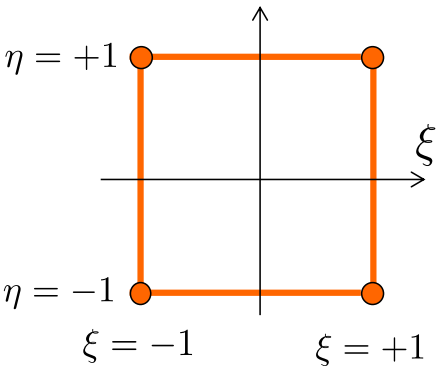
\includegraphics[width=0.3\textwidth]{figures/2Dquadrilateral.png}
		\caption{2D quadrilateral element.}
		\label{fig:2Dquadrilateral}
	\end{figure}
	First, lets consider linear shape functions ${}^e h_i \sim f(1,\xi,\eta,\xi\eta)$. A derivative of the shape function with respect to local coordinates is of order $\partial_{\xi,\eta} {}^e h_i \sim f(1,\xi,\eta)$. The computation of the element stiffness matrix ${}^e \matr{K}$ involves products of the derivatives of the shape functions, hence one has a function $\partial_{\xi,\eta} {}^e h_i \partial_{\xi,\eta} {}^e h_j \sim f(1,\xi,\eta,\xi^2,\eta^2,\xi\eta)$. The highest order terms to integrate via Gauss quadrature are hence quadratic, that is $k=2$. Therefore we need at least $(k+1)/2 = (2+1)/2 = 3/2$ and hence 2 integration points per axis for full integration. That is, in the case of a quadrilateral 2D element with linear shape functions, one has to have $2\times 2 = 2$ integration points per element to have full (exact) integration using Gauss quadrature. In case of quadratic shape functions for a 2D quadrilateral element, one will find that the highest order terms to integrate are of oder $k=4$. Hence one needs at least $(k+1)/2 = (4+1)/2 = 5/2$ and hence 3 integration point per axis and therefore $3\times 3 = 9$ integration points per element to have exact integration.
}


\section{Various questions}
\Que{What are contact problems?}
\Ans{
A contact problem is a situation in which there are two bodies with different properties interacting with each other. At the contact surface, the material properties are discontinuous. The challenge in contact problems is that contact may only occur in certain special circumstances; but if contact is established, many properties of the modelled system can change. For example, the conductance properties suddenly change when contact between surfaces is established.

Contact between two bodies typically feature \begin{itemize}
	\item contact pressure resisting penetration,
	\item frictional stress resisting sliding aswell as
	\item electrical and thermal interactions.
\end{itemize} Recall that stress is defined as internal force per area and strain is defined as deformation in the loaded condition relative to the unloaded situation.% lec 11
}

\Que{How does the FEM formulation to solve contact problems look like?.}
\Que{
Consider the usual formulation of a finite element problem:
\begin{equation}
	\matr{K}\vect{u} = \vect{F},
\end{equation} where $\vect{F}$ is the external force vector, $\vect{u}$ is the vector of nodal displacements and $\matr{K}$ is the stiffness matrix of the problem. The total potential energy for such a system involving contact surfaces is given by \begin{equation}
W(\vect{\lambda}, \vect{u}) = \frac{1}{2}\vect{u}^\top \matr{K}\vect{u} - \vect{u}^\top \vect{F} + \vect{\lambda}^\top\left(\vect{u}\matr{G}^\top-\vect{g}_0\right),
\end{equation} where $\matr{G}\vect{\lambda}$ are additional internal forces due to contact constraints, $\vect{\lambda}$ are Lagrange multipliers interpreted as contact forces and $\vect{g}_0$ is the desired gap between contact surfaces (usually 0 for perfect contact). Equilibrium conditions now require the gradients of the energy functional $W(\vect{\lambda},\vect{u})$ to be zero, hence \begin{equation}
\vect{\nabla}_{\vect{u}} W(\vect{\lambda}, \vect{u}) = \matr{K}\vect{u} - \vect{F} + \matr{G}\vect{\lambda} = 0, \quad \vect{\nabla}_{\vect{\lambda}} W(\vect{\lambda}, \vect{u}) = \matr{G}^\top \vect{u} - \vect{g}_0 = 0.
\end{equation} Combining both equations one gets \begin{equation}
\matr{K}\vect{u} + \matr{G}\vect{\lambda} = \vect{F}, \quad \matr{G}^\top \vect{u}=\vect{g}_0
\end{equation} and thus in matrix form \begin{equation}
\begin{pmatrix}
	\matr{K} & \matr{G} \\ \matr{G}^\top & \matr{0}  \end{pmatrix}\begin{pmatrix}
		\vect{u} \\ \vect{\lambda}
	\end{pmatrix} = \begin{pmatrix}
	\vect{F} \\ \vect{g}_0
	\end{pmatrix}.
\end{equation} One can see that it yields a new matrix equation of the same form as before: Stiffness matrix times displacement vector equals force vector.% lec 11
}

\Que{What are possible problems associated with solving contact problems?}
\Ans{
Solving contact problems with the finite element method is challenging for a number of reasons. First of all, contact between bodies of different material composition introduces geometrical aswell as material nonlinearities. Second, solutions tend to become unstable and iterative solvers may not converge easily anymore, because of non-smooth constraints. At a contact surface, the material properties for example can make jumps and thus the constraints are non-smooth. Lastly, the accuracy and robustness of the contact formulation can be highly mesh-dependent. % lec 11
}

\Que{What is the Lagrangian formulation of a finite element methods problem?}
\Ans{
The Lagrangian formulation is such that the nodes are fixed within the material and thus follow material deformation. The elements therefore deform as the material deforms.

Let $\vect{X}$ be the initial position of particles in a material and let $t$ be the time. Let furthermore $\vect{x}$ be the position of a particle initially at $\vect{X}$ at time $t=0$. In the Lagrangian formulation, the position of a particle at a later time $t$ is given by \begin{equation}
	\vect{x} = \vect{x}(\vect{X},t)
\end{equation} and thus the displacement is \begin{equation}
\vect{u}(\vect{X},t) = \vect{x}(\vect{X},t) - \vect{X}.
\end{equation} This corresponds to the coordinates (nodes) following material deformation.% lec 12
}

\Que{What is the Eulerian formulation of a finite element methods problem?}
\Ans{
The Eulerian formulation is such that the nodes are fixed in space and thus do not follow material deformation. The elements thus do not deform as the material deforms, rather the material flows through the elements.

Let $\vect{X}$ be the initial position of particles in a material and let $t$ be the time. Let furthermore $\vect{x}$ be the position of a particle initially at $\vect{X}$ at time $t=0$. In the Eulerian formulation, the position of a particle at a later time $t$ is given by \begin{equation}
	\vect{X} = \vect{X}(\vect{x},t)
\end{equation} and thus the displacement is \begin{equation}
	\vect{u}(\vect{x},t) = \vect{x} - \vect{X}(\vect{x},t).
\end{equation} This corresponds to the coordinates (nodes) being fixed in space and the material moving through the elements. % lec 12
}

\Que{What are the advantages and disadvantages of the Eulerian vs. the Lagrangian finite element method formulations?}
\Ans{
	In the Lagrangian formulation, the independent variables are the fixed positions $\vect{X}$ and the time $t$. The advantages of the Lagrangian formulation hence lie in accurate tracking of material interfaces, which is good for solid mechanics. When there are large deformations however, the mesh can distort tragically, because the coordinate system comoves with material deformation.
	
	In the Eulerian formulation, the independent variables are the material $\vect{x}$ positions and the time $t$. The advantage of the Eulerian formulation hence is that there is no mesh distortion, since elements stay fixed. The Eulerian formulation is therefore suitable for fluid flow and very large deformations. However, it is difficult to track material boundaries with this setup.  % lec 12
}

\Que{What is hyperelasticity? What is the difference to normal elasticity?}
\Ans{
E normal elastic material is characterized by a linear relationship between stress $\sigma$ and strain $\varepsilon$. Recall that stress is defined as internal force per area and strain is defined as deformation in the loaded condition relative to the unloaded situation. So in a normal elastic situation, one usually has a linear relationship $\sigma = E\varepsilon$, where $E$ is often Young's modulus, which is defined as the ratio of axial stress to axial strain. This situation is known as elastic condition and it is sufficient, if one only has relatively small deformations.

Hyperelasticity however occurs, when one has large elastic deformations such as in rubber or biological tissues. Energy is stored in the material, when it is being deformed. Hyperelasticity no longer features a linear relationship between stress and strain, which is the main difference between elasticity and hyperelasticity. % lec 13
}

\Que{What is parameter identification and how does a typical workflow using FEM software to do this look like?}
\Ans{
Parameter identification refers to a technique involving finite element software to determine the material properties (parameters) of a material. Consider some material and a model that is parametrized with material parameters $\vect{\theta} = (\theta_1,\dots,\theta_n)$. In order to determine the material parameters $\vect{\theta}$, one has to design an experiment, which can also be modelled in finite element software.

Let now $u$ be the observed quantity in the experiment. In the finite element model, the observed quantity is dependent upon the material parameters $\vect{\theta}$, therefore we write $u^{fem}(\vect{\theta})$. Furthermore, $u^{fem}_i(\vect{\theta})$ shall denote the value of the quantity $u(\vect{\theta})$ at the $i$'th measurement point out of $N$ in total. The measured experimental data we denote as $u_i^{exp}$.

Now, one defines initial parameters $\vect{\theta}_0$ and calculates the outcome of the experiment in a region $[\vect{\theta}_0 -\delta \vect{\theta}, \vect{\theta}_0 + \delta \vect{\theta}]$ using the finite element model. In order to have a measure on how appropriate the chosen parameters $\vect{\theta}$ are, one can define an objective function as \begin{equation}
	J(\vect{\theta}) = \sum_{i=1}^{N} \left(u_i^{fem}(\vect{\theta}) - u_i^{exp}\right)^2.
\end{equation} This objective function is to be minimized with respect to the model parameters $\vect{\theta}$. Calculating the gradient $\vect{\nabla}_{\vect{\theta}} J(\vect{\theta})$ can help to see in which direction the parameters $\vect{\theta}_i \rightarrow \vect{\theta}_{i+1}$ should be updated. Reiterate this procedure until convergence. In terms of a workflow, the procedure can be formulated as follows:
\begin{enumerate}
	\item Define a parametrized material model giving predicted data $u_i^{fem}(\vect{\theta})$.
	\item Conduct the simulated experiment in real live and gather data $u_i^{exp}$.
	\item Calculate predictions with finite element model using initial values $\vect{\theta}_0$.
	\item Reiterate model parameters $\vect{\theta}_j$ until one has $J(\vect{\theta}_{j+1})-J(\vect{\theta}_j) \rightarrow 0$.
\end{enumerate}% lec 13
}

\Que{What is a natural frequency?}
\Ans{
Consider the equation of motion for an undamped harmonic oscillator without forcing terms: \begin{equation}
	m\ddot{x}(t) + kx(t) = 0.
\end{equation} Here, $m$ is the mass of the oscillating point, $x(t)$ is the position of it and $k$ is the elasticity of the spring material. Now, assuming a solution of the form $x(t) = Ae^{i\omega t}$, the solution needs to fulfill \begin{equation}
-m\omega^2 A e^{i\omega t} + kAe^{i\omega t} = 0 \quad \Leftrightarrow \quad (k-m\omega^2)Ae^{i\omega t} = 0.
\end{equation} The amplitude $A$ and the exponential cannot be zero, hence the solution must fulfill \begin{equation}
\omega = \pm \sqrt{\frac{k}{m}} \doteq \omega_0,
\end{equation} which is called the natural frequency of the oscillator. This is the frequency at which this undamped and forcing-free oscillates. It can be shown that exciting a system at one of its natural frequencies leads to resonance, i. e. to ideal absorption of energy and hence to catastrophic outcomes on the system.
}

\Que{What is a resonance frequency?}
\Ans{
	In the context of mechanical or structural dynamics, the resonance frequency is the frequency at which a system oscillates with the maximum amplitude in response to an external periodic excitation. This phenomenon occurs when the frequency of the external force matches the system’s natural frequency, leading to constructive interference and energy accumulation over time.
	
	Let us derive the governing equation for the amplitude of a one-degree-of-freedom damped harmonic oscillator under harmonic forcing, and explain how resonance emerges.
	
	The starting point is the equation of motion for a mass-spring-damper system subjected to a sinusoidal driving force:
	\begin{equation}
		m\ddot{x}(t) + c\dot{x}(t) + kx(t) = F_0 \cos(\omega t),
	\end{equation}
	where $m$ is the mass, $c$ is the damping coefficient, $k$ is the stiffness, $F_0$ is the amplitude of the driving force, $\omega$ is the driving frequency and $x(t)$ is the displacement of the mass.
	
	To find the steady-state solution, we assume a particular solution of the form
	\begin{equation}
		x_p(t) = A(\omega)\cos(\omega t - \phi),
	\end{equation}
	where $A(\omega)$ is the frequency-dependent amplitude and $\phi$ is the phase shift.
	
	To solve this, we use the complex exponential form of the forcing function:
	\begin{equation}
		m\ddot{x}(t) + c\dot{x}(t) + kx(t) = \Re\{F_0 e^{i\omega t}\}.
	\end{equation}
	Assuming a complex solution of the form \( x(t) = \Re\{X(\omega) e^{i\omega t}\} \), where \( X(\omega) \in \mathbb{C} \), substitution into the equation of motion leads to
	\begin{align}
		 -m\omega^2 X(\omega)e^{i\omega t} + ic\omega X(\omega)e^{i\omega t} + k X(\omega)e^{i\omega t} = F_0 e^{i\omega t}
	\end{align} which is simplified to \begin{equation}
	X(\omega) = \frac{F_0}{k-m\omega^2 + ic\omega}.
	\end{equation}
	
	The amplitude is the modulus of this complex function:
	\begin{equation}
		A(\omega) = |X(\omega)| = \left| \frac{F_0}{k - m\omega^2 + i c\omega} \right| = \frac{F_0}{\sqrt{(k - m\omega^2)^2 + (c\omega)^2}}.
	\end{equation}
	Define the undamped natural frequency \( \omega_0 = \sqrt{\frac{k}{m}} \) and damping ratio \( \beta = \frac{c}{2m} \), the amplitude becomes:
	\begin{equation}
		A(\omega) = \frac{F_0/m}{\sqrt{(\omega_0^2 - \omega^2)^2 + (2\beta\omega)^2}}.
	\end{equation}
	
	The resonance frequency \( \omega_r \) is the frequency at which this amplitude \( A(\omega) \) is maximal. For weak damping (\( \beta \ll \omega_0 \)), the maximum occurs approximately at
	\begin{equation}
		\omega_r \approx \omega_0 = \sqrt{\frac{k}{m}}.
	\end{equation}
	At this frequency, the system absorbs energy most efficiently, resulting in oscillations of maximum amplitude. In practice, slight damping shifts the resonance peak to a frequency slightly less than \( \omega_0 \), and limits the amplitude from becoming unbounded.
}


\Que{How is the governing equation to calculate resonance frequencies for a FEM problem derived?}
\Ans{
Let us consider a one-dimensional, time- and space-dependent structural problem governed by the second-order partial differential equation (PDE)
\begin{equation}
	\rho(x) \frac{\partial^2 u(x,t)}{\partial t^2} - \frac{\partial}{\partial x}\left(E(x)\frac{\partial u(x,t)}{\partial x}\right) = f(x,t), \quad x \in [0,L] = \Omega, \quad t > 0
\end{equation}
subject to Dirichlet boundary conditions
\begin{equation}
	u(0,t) = u_{x0}, \quad u(L, t) = u_{xL}, \quad t > 0,
\end{equation}
and initial conditions
\begin{equation}
	u(x,0) = u_{t0}(x), \quad \frac{\partial u(x,0)}{\partial t} = v_{t0}(x).
\end{equation}
This is the strong form of the structural dynamics problem. In order to obtain a numerical solution, we must convert it to the weak form. This is done by multiplying both sides of the PDE with a weighting function $\delta u(x,t)$ and integrating over the domain $\Omega$:
\begin{equation}
	\int_\Omega \rho(x) \frac{\partial^2 u(x,t)}{\partial t^2}\delta u(x,t)\,\mathrm{d}x - \int_\Omega \frac{\partial}{\partial x}\left(E(x)\frac{\partial u(x,t)}{\partial x}\right)\delta u(x,t)\,\mathrm{d}x = \int_\Omega f(x,t)\delta u(x,t)\,\mathrm{d}x.
\end{equation}
Using integration by parts on the second term and assuming $\delta u(x,t)$ vanishes at the boundaries, we obtain
\begin{equation}
	\int_\Omega \rho(x) \frac{\partial^2 u(x,t)}{\partial t^2} \delta u(x,t)\,\mathrm{d}x + \int_\Omega E(x)\frac{\partial u(x,t)}{\partial x}\frac{\partial \delta u(x,t)}{\partial x}\,\mathrm{d}x = \int_\Omega f(x,t)\delta u(x,t)\,\mathrm{d}x.
\end{equation}
Next, we approximate the displacement $u(x,t)$ by a finite-dimensional hypothesis function $u^h(x,t)$:
\begin{equation}
	u^h(x,t) = \vect{H}(x)\vect{q}(t), \quad \delta u^h(x,t) = \vect{H}(x)\delta\vect{q}(t),
\end{equation}
where $\vect{H}(x) = (h_1(x),\dots,h_n(x))$ are global shape functions and $\vect{q}(t) = (q_1(t),\dots,q_n(t))^\top$ are the nodal unknowns. Inserting this into the weak form yields
\begin{equation}
	\int_\Omega \rho(x) \vect{H}(x)^\top \vect{H}(x)\,\mathrm{d}x \cdot \ddot{\vect{q}}(t) + \int_\Omega E(x)\frac{\mathrm{d}\vect{H}(x)^\top}{\mathrm{d}x} \frac{\mathrm{d}\vect{H}(x)}{\mathrm{d}x} \,\mathrm{d}x \cdot \vect{q}(t) = \int_\Omega f(x,t)\vect{H}(x)^\top\,\mathrm{d}x.
\end{equation}
We define the global system matrices and load vector as
\begin{align}\small\begin{aligned}
		\matr{M} &\doteq \int_\Omega \rho(x)\vect{H}(x)^\top\vect{H}(x)\,\mathrm{d}x, \quad
		\matr{K} \doteq \int_\Omega E(x)\frac{\mathrm{d}\vect{H}(x)^\top}{\mathrm{d}x} \frac{\mathrm{d}\vect{H}(x)}{\mathrm{d}x}\,\mathrm{d}x, \\
		\vect{r}(t) &\doteq \int_\Omega f(x,t)\vect{H}(x)^\top\,\mathrm{d}x,
\end{aligned}\end{align}
so the resulting semi-discrete system becomes
\begin{equation}\label{eq:structdynglobalsystem}
	\matr{M}\ddot{\vect{q}}(t) + \matr{K}\vect{q}(t) = \vect{r}(t).
\end{equation}
This equation represents the equation of motion for the 1D structural dynamics problem in the finite element framework. Time discretization of \cref{eq:structdynglobalsystem} leads to various explicit or implicit time-stepping schemes, depending on accuracy and stability requirements.
}

\Que{How are resonance frequencies calculated using the eigenvalue method in FEM problems?}
\Ans{
Recall, that in the case one wants to calculate resonance frequencies for some structural dynamics problem with the finite element method, the problem to solve is \begin{equation}
	\matr{M}\ddot{\vect{q}}(t) + \matr{K}\vect{q}(t) = \vect{r}(t),
\end{equation} where $\vect{r}(t)$ is the external forcing vector - which comprises for example of effects such as energy supplied to the oscillating system -, $\matr{K}$ is the stiffness matrix and $\matr{M}$ is the mass matrix of the problem. Furthermore, $\vect{q}(t)$ is the vector containing all position information for all nodes in the problem.

Now, in the case of calculating the natural frequencies - also known as the eigenfrequencies - of the system, the external forcing term is set to zero, i. e. $\vect{r}(t) = 0$. If that were not be the case, the resulting oscillating frequency would be determined or at leas influenced by the periodicity of $\vect{r}(t)$. The resulting equation to solve is hence \begin{equation}\label{eq:resonancefrequencyequation}
	\matr{M} \ddot{\vect{q}}(t) + \matr{K}\vect{q}(t) = 0.
\end{equation} Either, one solves this system via time-integration using explicit or implicit methods and extracts the frequency components via Fourier transformation from the obtained solution $\vect{q}(t)$; or one performs eigenvalue calculation. The latter strategy shall be briefly explained below.

Assume, that $\vect{q}(t)$ as a solution of the form \begin{equation}
	\vect{q}(t) = \vect{\phi}e^{i\omega t},
\end{equation} where $\omega$ is a possible natural frequency of the system. Now, inserting this into \cref{eq:resonancefrequencyequation} leads to \begin{equation}
-\omega^2 \matr{M}\vect{\phi}e^{i\omega t} + \matr{K}\vect{\phi}e^{i\omega t} = 0 \quad \Leftrightarrow \quad \left(\matr{K}-\omega^2\matr{M}\right)\vect{q}(t) = 0.
\end{equation} One can now go about using the Cholesky decomposition. The Cholesky decomposition theorem states, that any symmetric and positive-definite matrix $\matr{A}$ can be decomposed as \begin{equation}
\matr{A} = \matr{B}\matr{B}^\top,
\end{equation} where $\matr{B}$ is a unique lower triangular matrix. A matrix $\matr{A}$ is symmetric, if $\matr{A} = \matr{A}^\top$ and it is furthermore positive-definite, if all eigenvalues $\lambda_i$ of $\matr{A}$ are positive, i. e. $\lambda_i > 0$. Now, the mass matrix $\matr{M}$ is symmetric by definition and in most cases also positive-definite. Assuming the necessary conditions, we write \begin{equation}
\matr{M} = \matr{L}\matr{L}^\top
\end{equation} for a lower triangular matrix $\matr{L}$. Writing now $\vect{q}(t) = (\vect{L}^\top)^{-1} \vect{y}$ for a vector $\vect{y}$, this leads to the equation \begin{equation}
\matr{K}(\vect{L}^\top)^{-1} \vect{y} = \omega^2\matr{M}(\vect{L}^\top)^{-1} \vect{y} = \omega^2 \matr{L}\vect{y}
\end{equation} because of $\matr{M} = \matr{L}\matr{L}^\top$ and $(\matr{L}^\top)^{-1}\matr{L}^\top = \matr{L}^\top(\matr{L}^\top)^{-1} = \matr{I}$, where $\matr{I}$ is the identity matrix. Multiplying the above equation with $\matr{L}^{-1}$ from the left and defining $\matr{L}^{-\top} \doteq (\matr{L}^\top)^{-1}$, one obtains \begin{equation}
\matr{L}^{-1}\matr{K}\matr{L}^{-\top} \vect{y} = \omega^2 \matr{I} \vect{y}.
\end{equation} Defining $\matr{Q} \doteq \matr{L}^{-1}\matr{K}\matr{L}^{-\top} $ and $\lambda \doteq \omega^2$, one can see that the above equation is the general eigenvalue calculation equation, namely \begin{equation}
\matr{Q}\vect{y} = \lambda \vect{y}.
\end{equation} The eigenvalues $\lambda_i$ are calculated by finding the roots of the characteristic polynomial $\det(\matr{Q}-\lambda_i \matr{I})$, namely by calculating \begin{equation}
\lambda_i \quad \text{such that} \quad \det(\matr{Q}-\lambda_i \matr{I}) = 0.
\end{equation} Due to the presupposed positive-definiteness of $\matr{M}$, all eigenvalues are positive, which means that the $i$ eigenfrequencies (or natural frequencies) $\omega_i$ are calculated form the eigenvalues $\lambda_i$ as $\omega_i = \sqrt{\lambda_i}$.
}

\Que{What is Young's modulus?}  
\Ans{  
	Young’s modulus \(E\) measures material stiffness, defined as the ratio of axial stress to axial strain under elastic conditions
	\begin{equation}  
		E = \frac{\sigma}{\varepsilon}  ,
	\end{equation}  
	where \( \sigma \) is axial stress and \( \varepsilon \) is axial strain. Higher \(E\) indicates stiffer materials. Its unit is Pascal (Pa).  
}

\Que{What is the von Mises stress and how is it calculated?}  
\Ans{  
	The von Mises stress \(\sigma_{vM}\) predicts yielding under complex loading. It is derived from distortion energy theory and is expressed as  
	\begin{equation}  
		\sigma_{vM} = \sqrt{\frac{1}{2} \left[ (\sigma_1 - \sigma_2)^2 + (\sigma_2 - \sigma_3)^2 + (\sigma_3 - \sigma_1)^2 \right]}  .
	\end{equation}  
	Or in terms of Cartesian stress components we can write 
	\begin{equation}  
		\sigma_{vM} = \sqrt{ \sigma_x^2 + \sigma_y^2 + \sigma_z^2 - \sigma_x \sigma_y - \sigma_y \sigma_z - \sigma_z \sigma_x + 3(\tau_{xy}^2 + \tau_{yz}^2 + \tau_{zx}^2) } . 
	\end{equation}  
	Yielding occurs when \(\sigma_{vM} \geq \sigma_y\), where \(\sigma_y\) is the yield stress.  
}

\Que{What is Poisson's ratio and its significance?}  
\Ans{  
	Poisson’s ratio \(\nu\) describes the relationship between axial and transverse strain under uniaxial loading  
	\begin{equation}  
		\nu = - \frac{\varepsilon_{\text{transverse}}}{\varepsilon_{\text{axial}}}  .
	\end{equation}  
	It typically ranges from 0 to 0.5.   
}

\Que{What are stress and strain and how are they defined?}  
\Ans{  
	Stress \(\sigma\) is the internal force per unit area  
	\begin{equation}  
		\sigma = \frac{F}{A}  .
	\end{equation}  
	In 3D, stress is represented by the stress tensor:  
	\begin{equation}  
		\boldsymbol{\sigma} =  
		\begin{bmatrix}  
			\sigma_{xx} & \tau_{xy} & \tau_{xz} \\  
			\tau_{yx} & \sigma_{yy} & \tau_{yz} \\  
			\tau_{zx} & \tau_{zy} & \sigma_{zz}  
		\end{bmatrix} . 
	\end{equation}  
	Strain \(\varepsilon\) measures relative deformation:  
	\begin{equation}  
		\varepsilon = \frac{\Delta L}{L}  .
	\end{equation}  
	The strain tensor for 3D includes normal and shear deformations:  
	\begin{equation}  
		\boldsymbol{\varepsilon} =  
		\begin{bmatrix}  
			\varepsilon_{xx} & \gamma_{xy}/2 & \gamma_{xz}/2 \\  
			\gamma_{xy}/2 & \varepsilon_{yy} & \gamma_{yz}/2 \\  
			\gamma_{xz}/2 & \gamma_{yz}/2 & \varepsilon_{zz}  
		\end{bmatrix}  .
	\end{equation}  
	Stress represents internal resistance, while strain quantifies deformation. Their relationship is governed by laws like Hooke’s law.  
}


\end{document}
